% PT_COLOR.tex -- Persistence Theory Chromatic System (SCS)
% A first-principles color space derived from the sieve of Eratosthenes
\documentclass[12pt,a4paper]{article}
\usepackage{../shared/pt-common}
\usepackage[margin=2.5cm]{geometry}
\usepackage{setspace}
\onehalfspacing

\title{The Sieve Color Space:\\
A First-Principles Color Space from the Sieve of Eratosthenes}
\author{Yan Senez}
\date{\today}

\providecommand{\qrel}{\ensuremath{q_{\mathrm{rel}}}}
\begin{document}
\maketitle

\begin{abstract}
We present the Sieve Color Space (SCS), an information-geometric
substrate for color derived from a single assumption ($s = 1/2$) on a
prime-gap dynamical system. The construction yields a zero-parameter
Fisher metric on a three-channel simplex whose channel weights
$\gamp{3} > \gamp{5} > \gamp{7}$ are computed, not fitted, and match
the L$>$M$>$S cone-bandwidth ordering.

\medskip\noindent\textbf{Honest performance on COMBVD ($n = 3813$).}
As a standalone zero-parameter metric, pure SCS sits \emph{below}
CIELAB globally ($r = 0.500$ vs $0.755$) --- expected, since the
Fisher metric is theoretically exact only at threshold. It wins in
two regimes: the dark region ($r = 0.625$ vs $0.558$ for $L^* < 25$,
where CIELAB's linear leg flattens sensitivity) and MacAdam ellipse
\emph{orientation} (18/25 wins with zero parameters against CIELAB's
three). Treated as an additive information channel on top of a
measured cortical model, SCS improves both CIECAM02-based hybrids
($r = 0.824$ vs CIELAB's $0.755$, six regressed weights) and
CIEDE2000 ($\Delta E_{\mathrm{SCS00}}$: $r = 0.893$ vs $0.878$,
$p < 0.0001$, five regressed weights). The hybrids use fitted
parameters and are labeled as such throughout the paper.

\medskip\noindent\textbf{Positioning.} SCS is proposed as a principled
geometric \emph{layer} in a factored color-appearance architecture ---
alongside iCAM (Fairchild \& Johnson, 2004), CAM02-UCS (Luo et al.,
2006), and J\textsubscript{z}A\textsubscript{z}B\textsubscript{z}
(Safdar et al., 2017) --- not as a replacement for the CIE toolkit.
Chromatic adaptation, spectral sensitivity beyond the HPE
linearization, viewing conditions, flare, and observer variability
are explicitly outside scope (\S\ref{sec:scope_limits}); CIECAM02 and
$\Delta E^*_{00}$ remain the appropriate tools where those effects
dominate.

\medskip\noindent\textbf{Open invitations.} Three falsifiable
predictions, each tractable in a three-month experiment, are stated
in \S\ref{sec:open_problems}: a Koide-saturation JND null at
$S/S_{\max} = 1/\sqrt{2}$; a CRT-driven chromatic-discrimination
ceiling at $3 \times 5 \times 7 = 105$ states; and a fourth-channel
signature from $p = 11$ in tetrachromats. Code, COMBVD splits,
MacAdam fits, and a public leaderboard are released at
\href{https://github.com/Igrekess/SieveColorSpace}{github.com/Igrekess/SieveColorSpace}.
We do not claim SCS is finished; we claim it is testable.
This article is self-contained: an appendix provides self-contained
derivations of the Persistence Theory results used --- forbidden sieve
transitions, the parameter $s = 1/2$, the sum rule, the vertex--edge
bifurcation, the holonomy identity, anomalous dimensions, the active
prime criterion, and the fixed point $\mustar = 15$ --- so that no
external reference is needed to verify the deductive chain.
\end{abstract}

\tableofcontents
\newpage

% ============================================================
\section{Relation to the CIE framework: what is derivable, what is measured}
\label{sec:intro}
% ============================================================

The Commission Internationale de l'\'Eclairage (CIE) framework ---
tristimulus $(X, Y, Z)$, chromaticity $(x, y)$, the 1976 CIELAB uniform
space, and the CIEDE2000 color-difference formula --- is the empirical
foundation of modern colorimetry. It works: it underwrites industrial
calibration, display manufacturing, medical imaging, and fifty years of
psychophysics. Any proposed substrate has to explain its own role
relative to this infrastructure, not against it.

Persistence Theory (PT) offers a \emph{complementary} geometric
substrate. The Sieve Color Space (SCS) constructed below derives, from
a single input ($s = 1/2$ on a prime-gap dynamical system), five
features that CIE takes as measured or design-chosen:

\begin{enumerate}[nosep]
\item \textbf{A derived metric.} CIELAB's cube-root nonlinearity is an
  empirical design choice. SCS proposes a Fisher-information metric on
  a three-channel probability simplex; the CIELAB cube root turns out
  to be a low-order approximation to the exact Bhattacharyya coordinate
  of this metric (\S\ref{sec:comparison}).
\item \textbf{A saturation--luminance sum rule.} CIE has no identity
  linking the two; SCS inherits $\DKL + H = \log 3$, a consequence of
  information-theoretic definitions applied to a three-outcome
  distribution (\S\ref{sec:scs}).
\item \textbf{Additive/subtractive as two branches.} The RGB/CMY duality
  is a practical convention in CIE. SCS reads it as two chiral branches
  of the sieve, each parametrized by a single angle $\theta_p$
  (\S\ref{sec:scs}).
\item \textbf{Three channels, and a hierarchy.} Trichromacy is a
  biological given in CIE. SCS derives that exactly three primes
  $\{3, 5, 7\}$ are active at $\mustar = 15$ and yields the strict
  ordering $\gamp{3} > \gamp{5} > \gamp{7}$ matching the L$>$M$>$S
  cone-bandwidth ordering (\S\ref{sec:foundation}).
\item \textbf{An optimal saturation point.} Perceptual preference
  studies cluster around $65$--$75\%$ of maximum saturation without a
  structural reason; SCS predicts a Koide equilibrium at
  $1/\sqrt{2} \approx 70.7\%$ and proposes a sharper forced-choice JND
  test to discriminate it from its neighborhood (\S\ref{sec:scs}).
\end{enumerate}

The standalone SCS metric does \emph{not} replace CIELAB: as a pure
geodesic with zero fitted parameters it sits below CIELAB globally on
COMBVD, and only outperforms CIELAB in specific regimes (dark region,
MacAdam ellipse orientation). Where SCS earns its weight is as an
\emph{additional information channel} on top of existing cortical
models: SCS\,+\,CIECAM02 surpasses CIELAB globally, and
$\Delta E_{\mathrm{SCS00}}$ (a fitted hybrid with CIEDE2000) surpasses
CIEDE2000 itself. The framing of this paper, and of the invitations in
\S\ref{sec:open_problems}, is this additive one. What SCS does not
model (chromatic adaptation, spectral sensitivity beyond HPE
linearization, viewing conditions, flare, observer variability) is
stated explicitly in \S\ref{sec:scope_limits}; CIECAM02 and CIEDE2000
remain the appropriate tools where those effects dominate.

\paragraph{Reading this paper without a commitment to the broader framework.}
SCS is a direct application of \emph{Persistence Theory} (PT) ---
a framework developed independently and with its own program,
outlined in the companion monograph~\cite{senez2026math}. This paper is
deliberately self-contained: we recall only the minimal PT results we
use ($s = 1/2$, the fixed point $\mustar = 15$, the active-prime
criterion), and we provide self-contained derivations of each in
Appendix~\ref{app:pt_proofs}. A colour scientist, information
geometer, or vision neuroscientist can read, evaluate, and extend the
claims below without accepting PT as a whole --- the only inputs the
reader has to accept are (i) that three primes $\{3, 5, 7\}$ are the
active channels, (ii) the three weights $\gamp{3}, \gamp{5}, \gamp{7}$
quoted in \S\ref{sec:foundation}, and (iii) the Fisher metric on the
simplex. Everything else in this paper follows from these inputs plus
standard information geometry and colorimetry. Whether or not PT is
the right story for why those three weights take those values is an
interesting question; it is not a question this paper asks the reader
to settle.

% ============================================================
\section{The Sieve Foundation: From $s = 1/2$ to $\{2, 3, 5, 7\}$}
\label{sec:foundation}
% ============================================================

We recall the minimal PT chain relevant to color. Full
self-contained proofs are given in Appendix~\ref{app:pt_proofs};
the reader wishing to verify every step may refer there without
consulting the monograph~\cite{senez2026math}.

\begin{theorembox}[T1: Forbidden transitions]
For any three consecutive primes $p, p', p''$ with $p > 3$, the gaps
$g = p'-p$ and $g' = p''-p'$ cannot both lie in the same nonzero
residue class mod~3. This forces the transfer matrix $T_3$ to have
structural zeros at $T_{11} = T_{22} = 0$, and the symmetry parameter
$s = 1/2$.
\end{theorembox}

From $s = 1/2$, the sieve dynamics converge (Theorems T4--T5) to a
unique fixed point $\mustar = 15$, at which the effective dimensions
$\gamp{p}$ satisfy:

\begin{identitybox}[Active primes at $\mustar = 15$]
\begin{align}
\gamp{3} &= 0.808 > 1/2 \quad \text{(active --- red channel)} \\
\gamp{5} &= 0.696 > 1/2 \quad \text{(active --- green channel)} \\
\gamp{7} &= 0.595 > 1/2 \quad \text{(active --- blue channel)} \\
\gamp{11} &= 0.427 < 1/2 \quad \text{(inactive)}
\end{align}
The threshold $1/2$ derives from $s = 1/2$. Exactly $\{3, 5, 7\}$
are active. \textsc{[thm, D08]}
\end{identitybox}

\begin{figure}[ht]
\centering
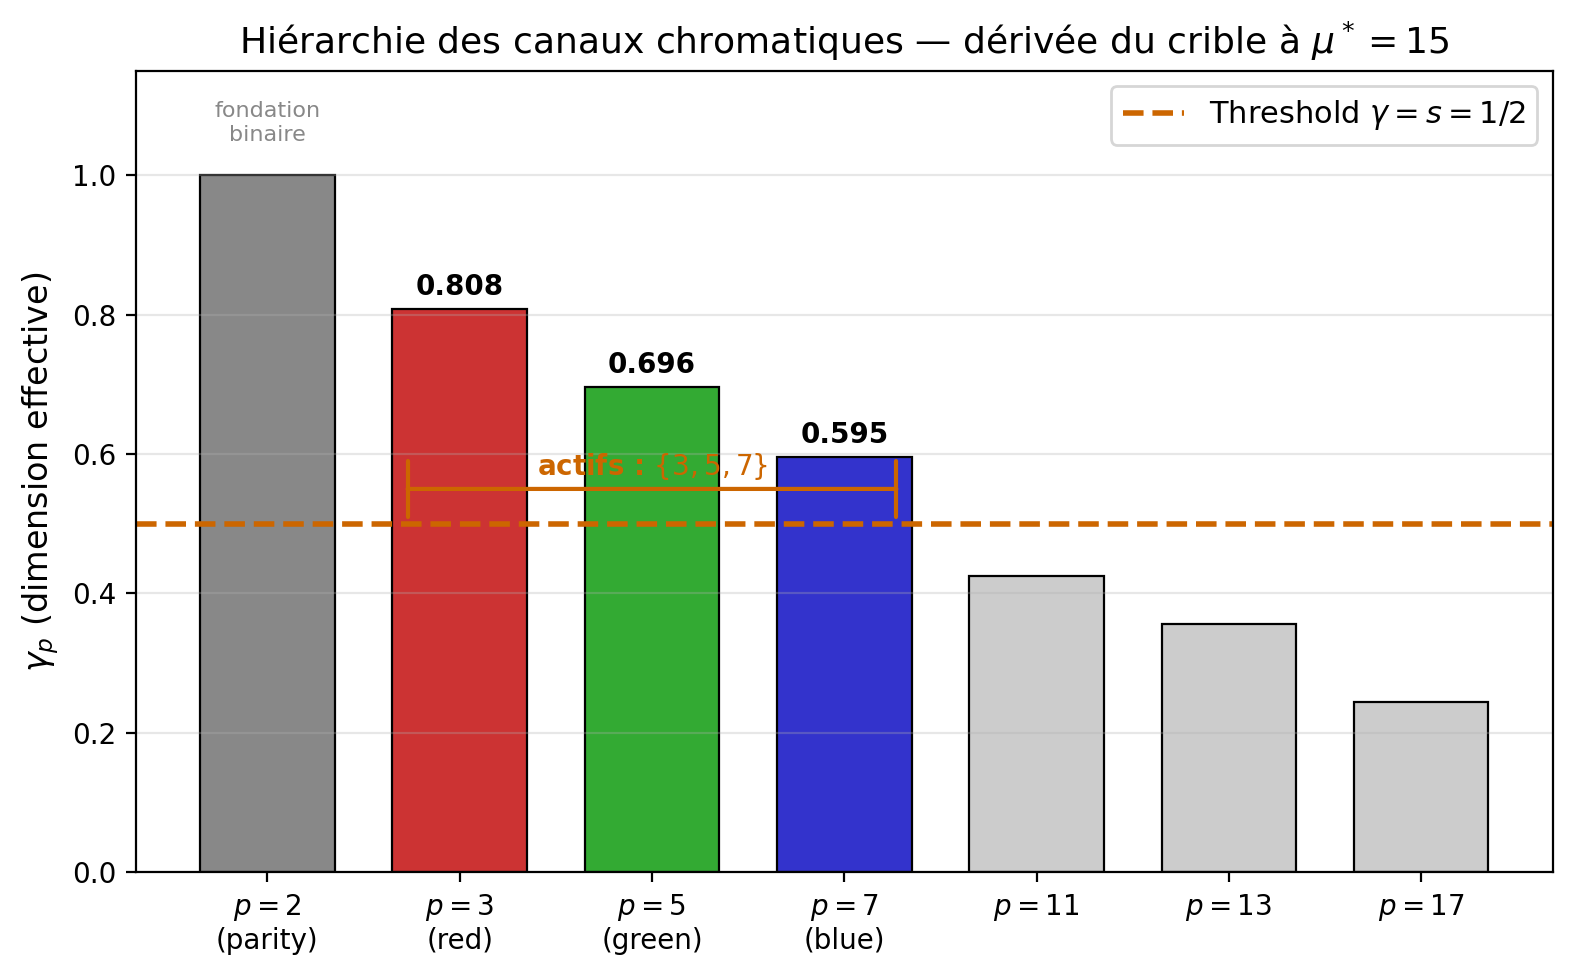
\includegraphics[width=0.8\textwidth]{figures_en/fig5_gamma_hierarchy.png}
\caption{Effective dimensions $\gamp{p}$ at $\mustar = 15$.
Only $\{3, 5, 7\}$ exceed the threshold $s = 1/2$ (orange dashed line).
The strict monotonicity $\gamp{3} > \gamp{5} > \gamp{7}$ determines
the cone hierarchy L $>$ M $>$ S.}
\label{fig:hierarchy}
\end{figure}

The prime $p = 2$ plays a structurally distinct role: it creates
\emph{parity} --- the binary distinction present/absent,
light/dark --- the foundation on which the three chromatic channels
are built. The complete structure is therefore $\{2, 3, 5, 7\}$:
\begin{equation}
  \underbrace{p = 2}_{\text{luminance (binary)}} \quad + \quad
  \underbrace{\{3, 5, 7\}}_{\text{chromaticity (ternary)}}
\end{equation}

% ============================================================
\section{The Sieve Color Space (SCS)}
\label{sec:scs}
% ============================================================

\subsection{Coordinates: the chromatic simplex $\Delta^2$}

\begin{figure}[ht]
\centering
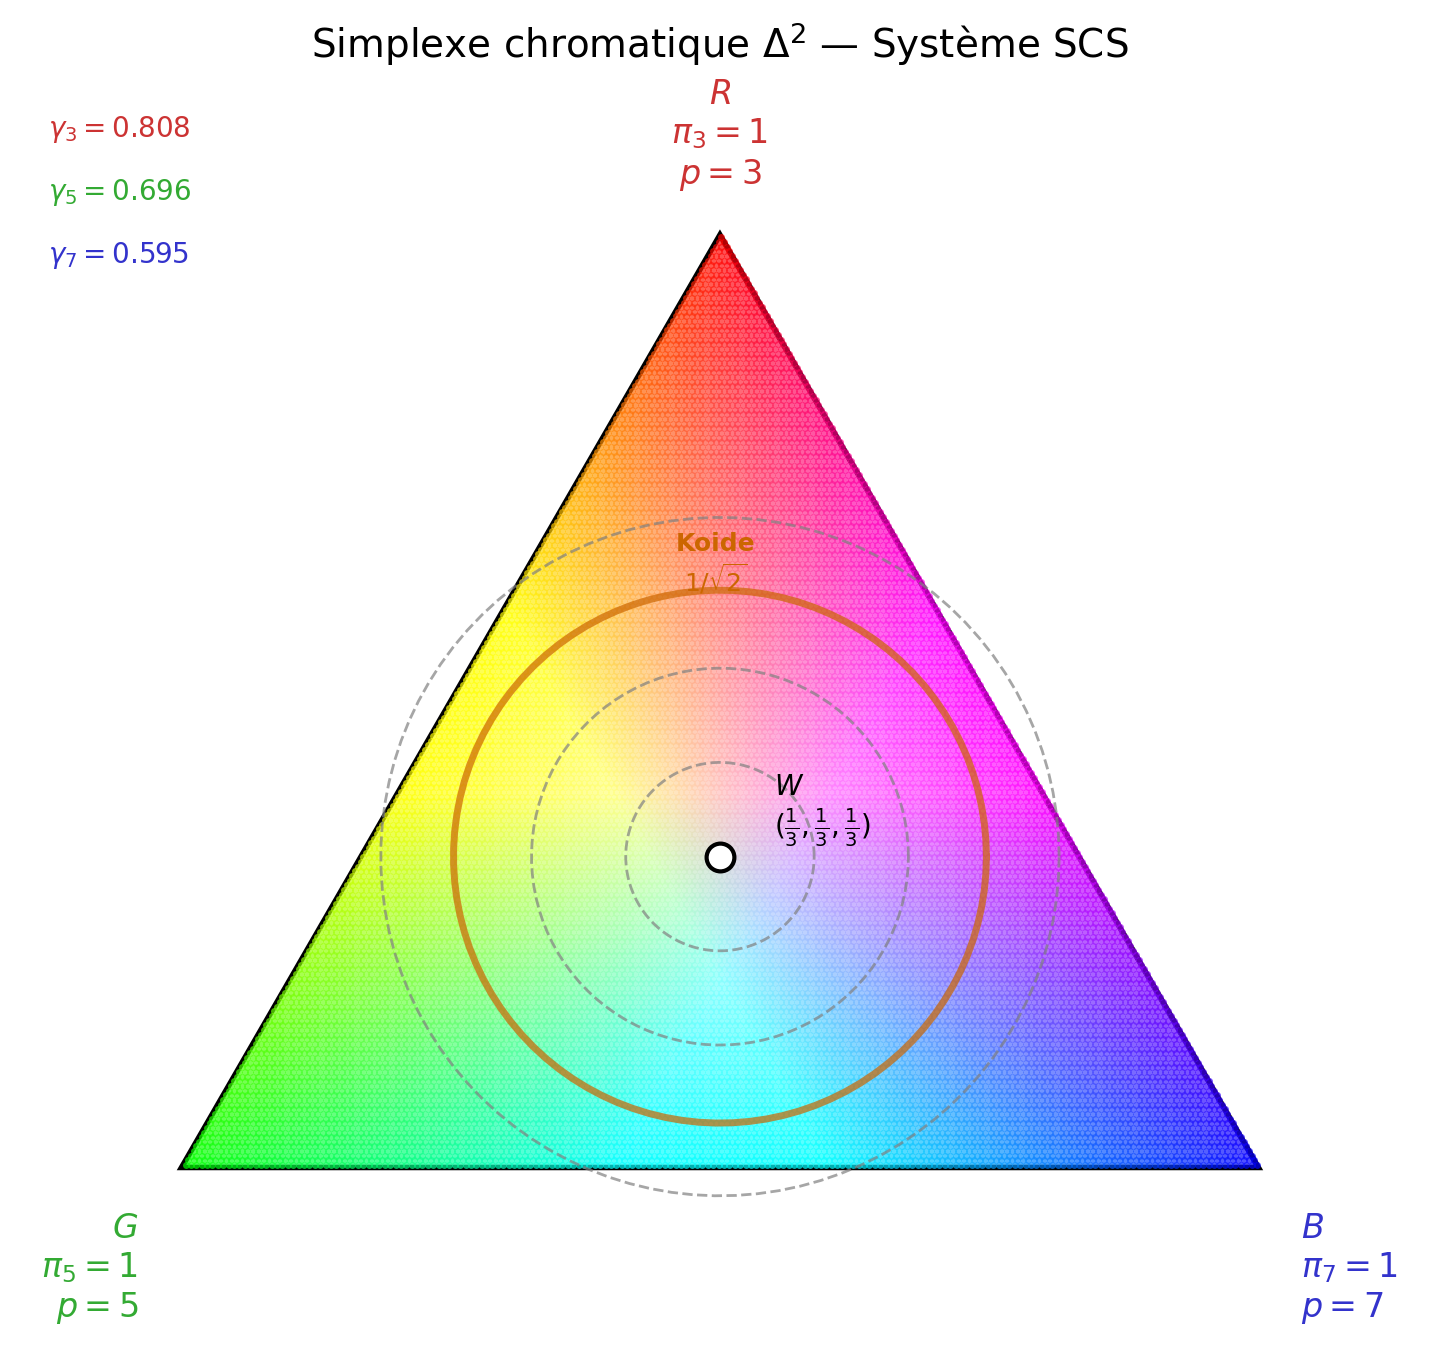
\includegraphics[width=0.75\textwidth]{figures_en/fig1_simplex.png}
\caption{The chromatic simplex $\Delta^2$ with vertices at the three
spectral primaries ($p=3,5,7$), white at the center, and iso-saturation
contours. The Koide equilibrium at $1/\sqrt{2} \approx 70.7\%$ is
marked in orange.}
\label{fig:simplex}
\end{figure}

A color is a probability distribution over the three active channels:
\begin{equation}
  \bm{\pi} = (\pi_3,\, \pi_5,\, \pi_7), \qquad
  \pi_3 + \pi_5 + \pi_7 = 1, \qquad \pi_p \geq 0.
  \label{eq:simplex}
\end{equation}

This is the 2-simplex $\Delta^2$ --- a triangle with vertices at the
three spectral primaries:
\begin{itemize}[nosep]
\item $R = (1,0,0)$: pure red (channel $p=3$ only)
\item $G = (0,1,0)$: pure green (channel $p=5$ only)
\item $B = (0,0,1)$: pure blue (channel $p=7$ only)
\item $W = (1/3, 1/3, 1/3)$: white (uniform distribution)
\end{itemize}

The luminance axis ($p = 2$) is orthogonal to $\Delta^2$. A full color
specification is $(\ell, \bm{\pi})$ where $\ell \in [0,1]$ is the
binary luminance level and $\bm{\pi} \in \Delta^2$ is the chromaticity.

\begin{remark}
The CIE chromaticity diagram $(x,y)$ is a projective transformation of
$\Delta^2$. The simplex coordinates $\bm{\pi}$ are the natural
(barycentric) coordinates; CIE's $(x,y)$ are a reparametrization that
obscures the underlying symmetry.
\end{remark}

\subsection{The metric: Fisher information weighted by $\gamp{p}$}

The fundamental question of color science is: \emph{how far apart are
two colors?} CIE has no principled answer. PT does.

\begin{theorembox}[\v{C}encov's theorem applied to $\Delta^2$]
On any statistical manifold, the Fisher information metric is the
\emph{unique} Riemannian metric (up to a constant) that is monotone
under sufficient statistics (Markov embeddings). On $\Delta^2$, this
metric is:
\begin{equation}
  ds^2 = \sum_{p \in \{3,5,7\}} \gamp{p} \,
    \frac{d\pi_p^2}{\pi_p}
  \label{eq:fisher}
\end{equation}
where $\gamp{p}$ are the effective dimensions at $\mustar = 15$.
\textsc{[thm]} --- \v{C}encov (1982), applied to the PT simplex.
\end{theorembox}

The weights $\gamp{p}$ are not fitted --- they are \emph{derived} from
the sieve dynamics. Their effect:

\begin{itemize}[nosep]
\item Near the green vertex ($\pi_5 \to 1$): $\gamp{5} = 0.696$ and
  $\pi_5$ is large, so $d\pi_5^2/\pi_5$ is small --- but $\gamp{5}$
  amplifies it. Net effect: \emph{maximal discrimination in the
  yellow-green zone}.
\item Near the blue vertex ($\pi_7 \to 1$): $\gamp{7} = 0.595$ is the
  smallest weight. Net effect: \emph{coarser discrimination in blue}.
\item Near the red vertex ($\pi_3 \to 1$): $\gamp{3} = 0.808$ is the
  largest weight. Net effect: \emph{wide-band sensitivity}.
\end{itemize}

This hierarchy $\gamp{3} > \gamp{5} > \gamp{7}$ matches the
\emph{ordering} of L, M, S cone bandwidths and produces a qualitative
pattern of MacAdam-like ellipse elongation. Quantitative ellipse
predictions are reported in \S\ref{sec:comparison}; the match is
ordinal here, not spectral.

\begin{figure}[ht]
\centering
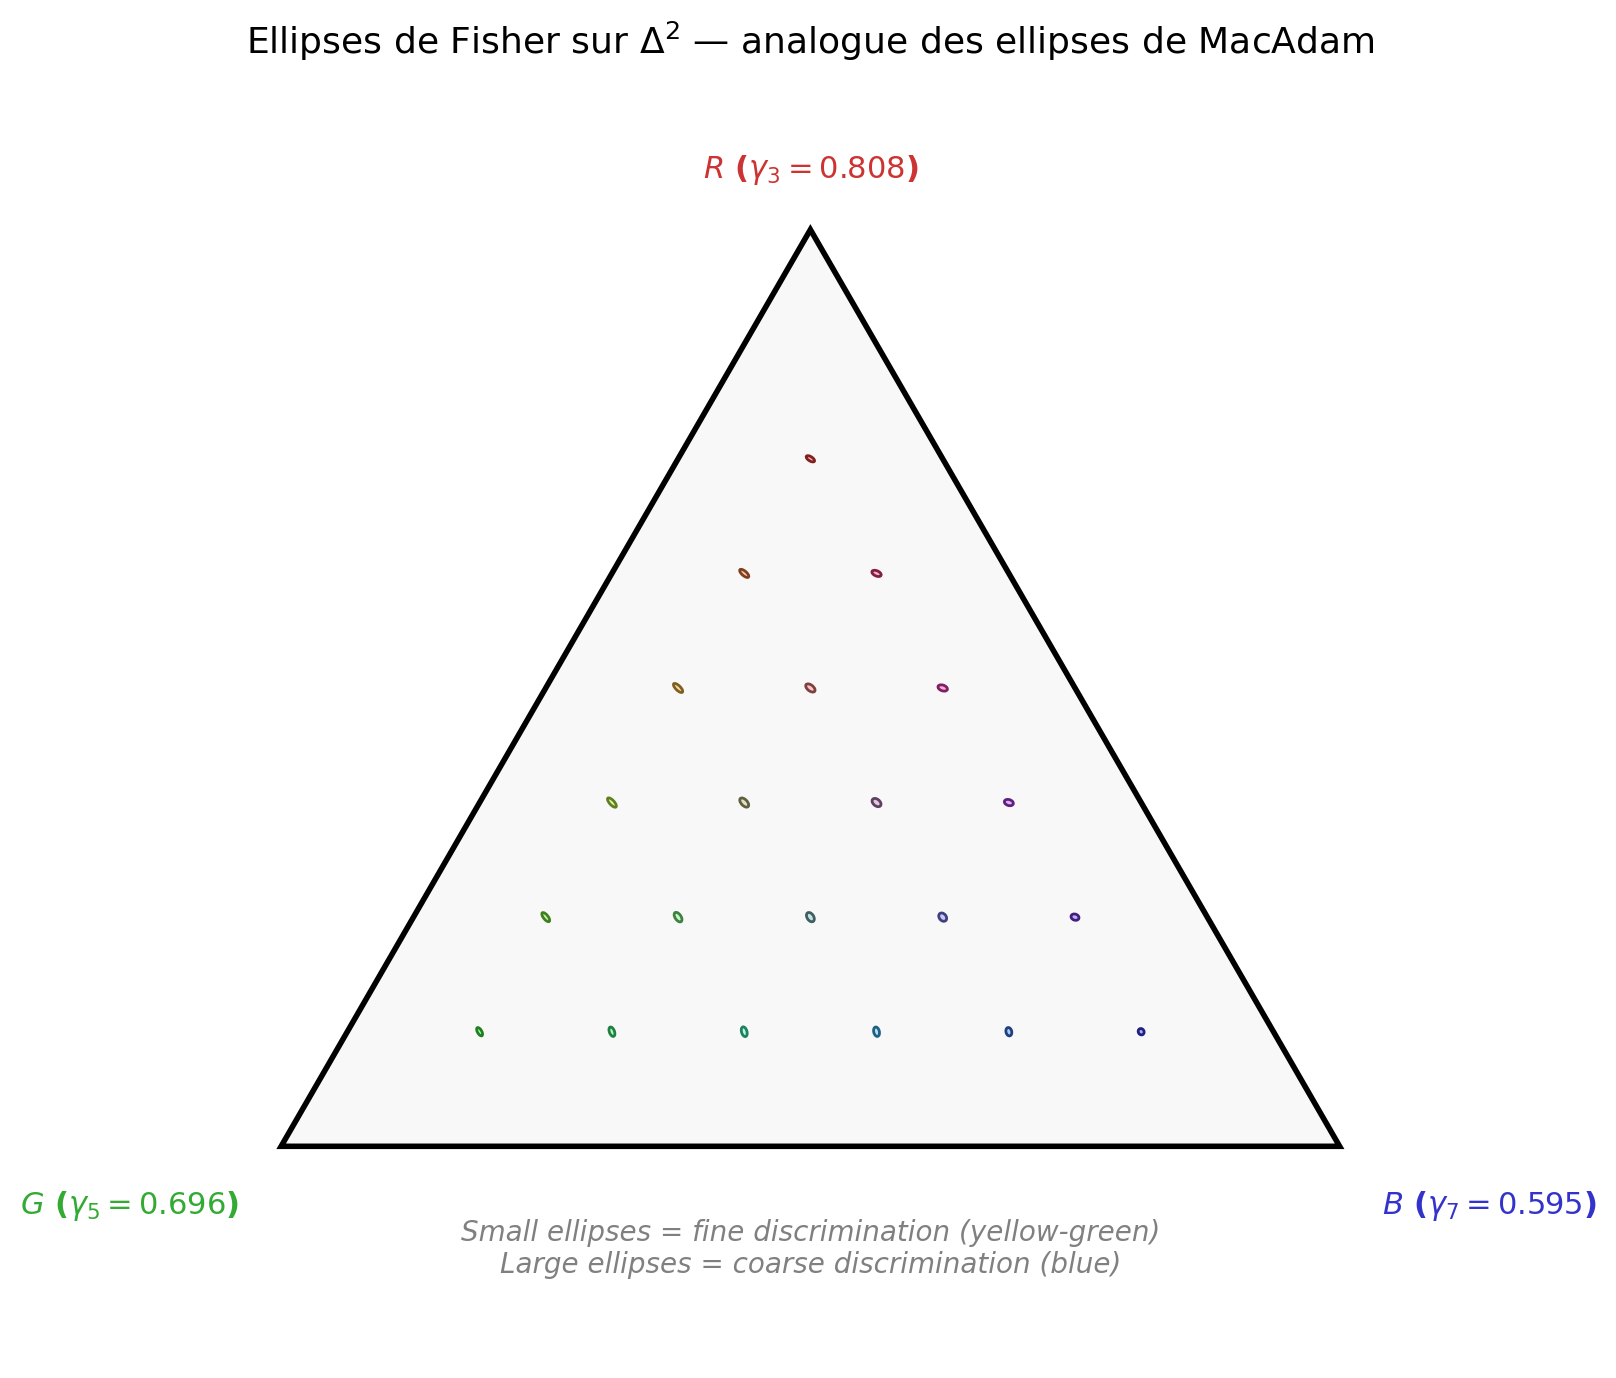
\includegraphics[width=0.75\textwidth]{figures_en/fig3_fisher_ellipses.png}
\caption{Fisher metric ellipses on $\Delta^2$. Small ellipses (green-yellow
zone) indicate fine discrimination; large ellipses (blue zone) indicate
coarser discrimination. Compare with MacAdam (1942).}
\label{fig:fisher}
\end{figure}

\subsection{Information-geometric status of SCS}
\label{sec:infogeo}

For readers from the information-geometry community, this subsection
states the formal status of the SCS metric in the language of Amari
and \v{C}encov, and points out where the construction departs from
standard information-geometric practice.

\paragraph{The manifold and its metric.}
The chromatic manifold is the open simplex
$\Delta^2 = \{\bm{\pi} \in \mathbb{R}^3_{>0} : \sum_p \pi_p = 1\}$
with $p \in \{3, 5, 7\}$. The Fisher information metric on
$\Delta^2$ is unique up to a positive constant by \v{C}encov's theorem
\cite{cencov1982}: any Riemannian metric on a statistical manifold
invariant under sufficient statistics is proportional to the Fisher
metric. \v{C}encov fixes the metric up to a global scale; it does
\emph{not} fix the per-coordinate weighting. The SCS construction
adds a weighted structure
\begin{equation}
  ds^2_{\mathrm{SCS}}
  = \sum_{p \in \{3,5,7\}} \gamp{p}\;\frac{d\pi_p^2}{\pi_p},
  \label{eq:scs_metric}
\end{equation}
with $\gamp{p}$ derived from the sieve at $\mustar = 15$. The
weighting breaks the invariance of the bare Fisher metric under
arbitrary relabelings of the three channels and introduces a
\emph{colour-specific structure} that \v{C}encov's theorem alone does
not supply. The SCS claim is precisely that the $\gamp{p}$ weighting
is the natural one for the colour simplex, not that \v{C}encov forces
it.

\paragraph{Dual connections and the $\alpha = 1/2$ choice.}
Amari's exponential family of connections $\nabla^{(\alpha)}$ on
$\Delta^2$ contains three standard points: $\alpha = 1$ (exponential,
$e$-connection), $\alpha = -1$ (mixture, $m$-connection), and
$\alpha = 0$ (the Levi-Civita connection of the Fisher metric, also
known as the $1/2$-connection in the Bhattacharyya parametrization).
The coordinate change $\xi_p = 2\sqrt{\gamp{p}\,\pi_p}$
(Eq.~\eqref{eq:bhattacharyya}) sends the SCS metric onto flat
Euclidean geometry, which identifies the \v{C}encov--Amari
$\alpha = 0$ connection as the one operative in the construction
(the Fisher--Rao geodesic between two distributions is
$2 \arccos \sum_p \sqrt{\pi_{1,p}\,\pi_{2,p}}$, which is the chordal
distance in $\xi$ coordinates).

\paragraph{Čencov $\to$ cone weighting: the open question.}
The content of SCS that is not \v{C}encov is the three specific
weights $\gamp{3}, \gamp{5}, \gamp{7}$ and their ordering. An
information-geometry reader will naturally ask: \emph{is there a
variational characterization of the $\gamp{p}$ weighting from first
principles on the simplex alone, or is the sieve providing information
that the simplex cannot?} Our current view is that the sieve
contributes information about \emph{which} distributions are physically
realizable (the three active primes at $\mustar = 15$ are a structural
input), not just the metric on them. A cleaner information-theoretic
characterization of this input --- perhaps as a prior over three-outcome
distributions satisfying a specific marginal constraint --- would be
a direct connection between this paper and the
variational-inference / conjugate-prior literature. We flag it as
open.

\paragraph{Relation to prior line-element theories.}
The SCS metric is a continuation of the line-element tradition in
colour science, starting with Helmholtz (1896), elaborated by
Schrödinger (1920), and refined by Stiles (1946), Vos and Walraven
\cite{voswalraven1972}, and Wyszecki and Stiles \cite{wyszecki2000}.
Those constructions typically build a Riemannian metric on
\emph{cone-contrast space} and fit the metric coefficients to
discrimination data (MacAdam, Brown, Wyszecki ellipses). SCS is
structurally simpler in one respect (zero fitted parameters) and
structurally narrower in another (it prescribes the weights via the
sieve rather than reading them off the data). A systematic
reproduction of the classical line-element results with SCS weights
substituted for fitted ones is a natural test we have not yet run;
it is part of experiment E3 in \S\ref{sec:open_problems}.

\subsection{Saturation: $\DKL$ divergence from white}

\begin{derivedbox}[Saturation as informational distance]
The saturation of a color $\bm{\pi}$ is its Kullback--Leibler
divergence from the achromatic point:
\begin{equation}
  S(\bm{\pi}) = \DKL(\bm{\pi} \,\|\, \mathbf{u})
    = \sum_{p} \pi_p \log(3\,\pi_p)
  \label{eq:saturation}
\end{equation}
where $\mathbf{u} = (1/3, 1/3, 1/3)$.

Saturation is zero at white and maximal ($\log 3$) at any spectral
primary. \textsc{[der]}
\end{derivedbox}

\subsection{Luminance: entropy of the chromatic distribution}

\begin{derivedbox}[Perceptual luminance as entropy]
The perceptual luminance within the chromatic plane is the Shannon
entropy of $\bm{\pi}$:
\begin{equation}
  L(\bm{\pi}) = H(\bm{\pi}) = -\sum_{p} \pi_p \log \pi_p
  \label{eq:luminance}
\end{equation}
$L$ is maximal at white ($\log 3$) and zero at any spectral primary.
\textsc{[der]}
\end{derivedbox}

\subsection{The $S + L$ sum rule: a generic identity on three outcomes}

\begin{identitybox}[Information-theoretic sum rule]
For any color $\bm{\pi} \in \Delta^2$:
\begin{equation}
  \boxed{\DKL(\bm{\pi} \,\|\, \mathbf{u}) + H(\bm{\pi}) = \log 3}
  \label{eq:gft}
\end{equation}
Equivalently: $S + L = \log 3$. \textsc{[id, D02]}
\end{identitybox}

\begin{remark}[Scope of this identity]
Equation~\eqref{eq:gft} is a generic algebraic identity: for any
probability distribution $\bm{\pi}$ on $n$ outcomes with uniform
reference $\mathbf{u}$,
$\DKL(\bm{\pi}\|\mathbf{u}) + H(\bm{\pi}) = \log n$. It holds whether
those $n$ outcomes are wavelengths, dice faces, or anything else. The
identity itself is \emph{not} a color law --- it is a consequence of
the definitions of $\DKL$ and $H$ applied to a uniform reference.
\emph{What is color-specific} in the present construction is the
choice of $n = 3$ (derived from the sieve via $\{3,5,7\}$), the
assignment of the three outcomes to the three active chromatic
channels, and the physical reading of $S$ as saturation and $L$ as
perceptual luminance within the chromatic plane. With those
identifications in place, the identity becomes a \emph{budget} linking
saturation and luminance: increasing one decreases the other. This is
substantive in that it constrains how the two quantities trade off,
but the algebraic content was never in doubt.
\end{remark}

\begin{remark}[Relation to the Gap Fundamental Theorem]
The SCS sum rule should not be conflated with the Gap Fundamental
Theorem (T2) of the PT monograph, which concerns the sieve transfer
matrix and is a non-trivial structural result. The color identity
\eqref{eq:gft} is a consequence of information-theoretic definitions;
its interpretation as a saturation--luminance budget is what is new
here.
\end{remark}

\begin{figure}[ht]
\centering
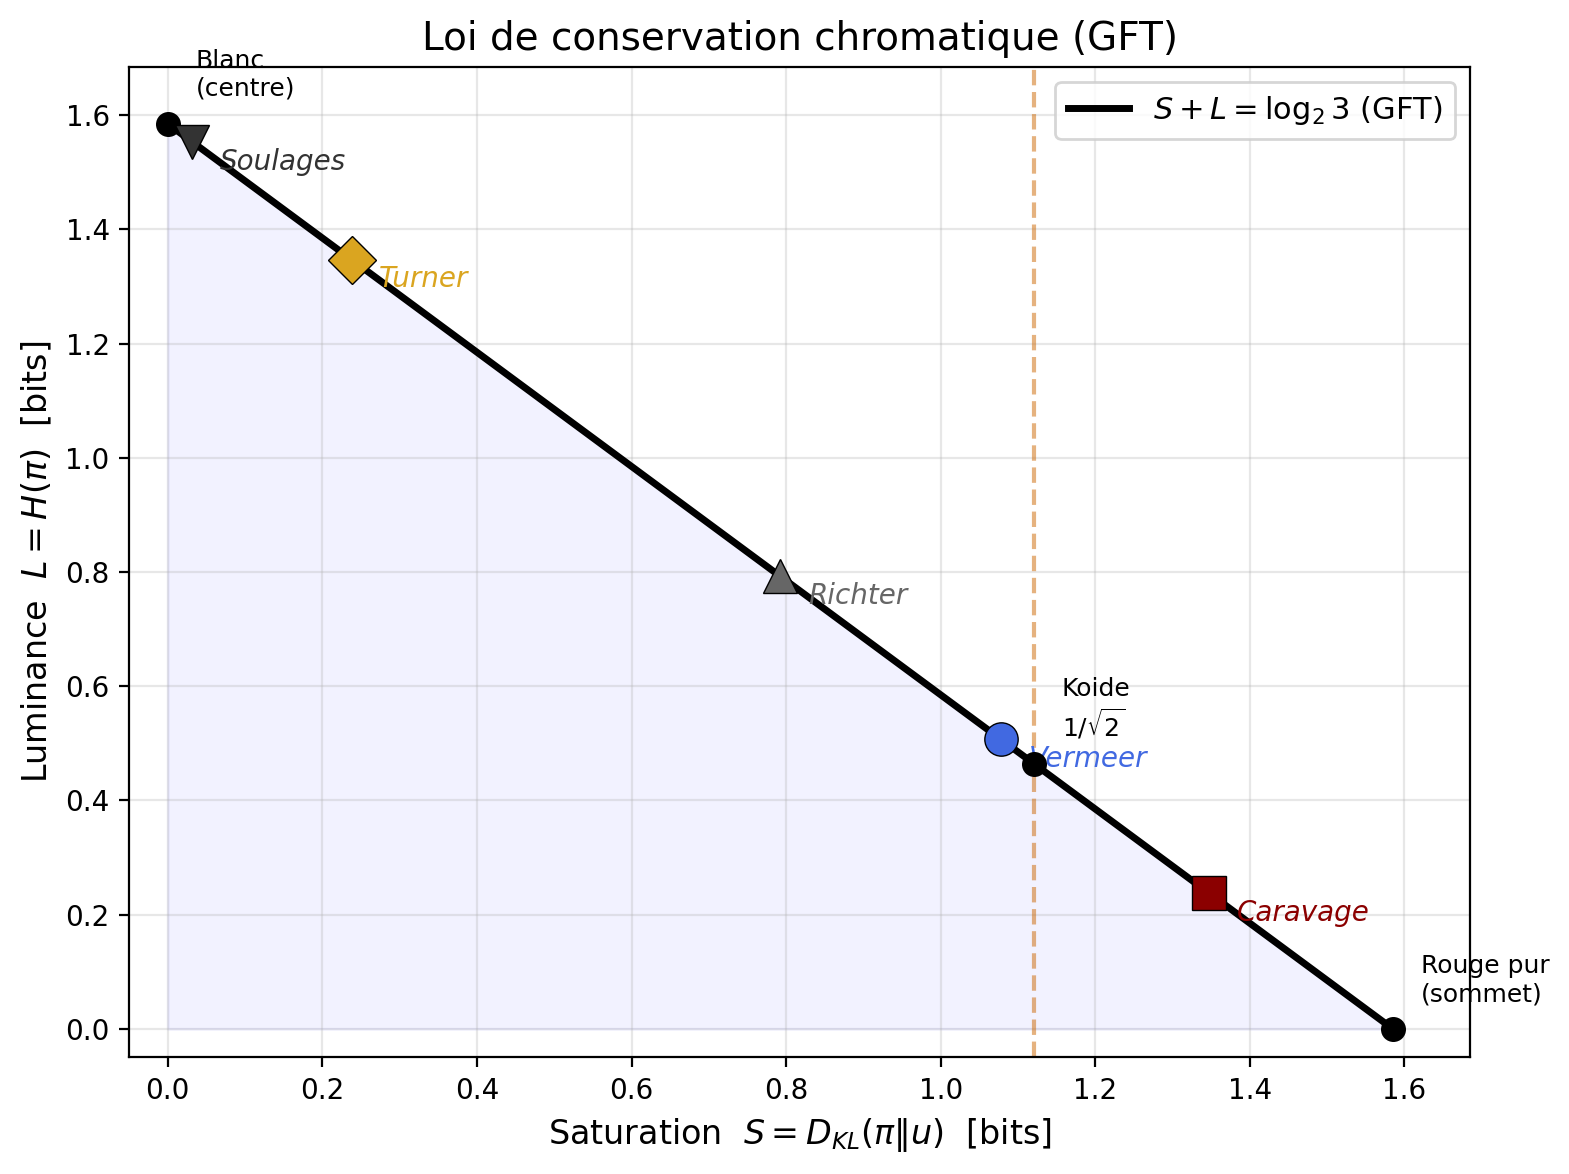
\includegraphics[width=0.8\textwidth]{figures_en/fig2_conservation.png}
\caption{The sum rule $S + L = \log 3$ (natural log). Every color lies on
this line. Artists choose \emph{where}: Caravage maximizes saturation
(dark contrasts), Turner maximizes luminance (dissolved light), Vermeer
works near the Koide point.}
\label{fig:conservation}
\end{figure}

\begin{remark}[Thermodynamic analogy, with the caveat made explicit]
The $S+L$ budget admits a loose analogy with the first law of
thermodynamics, $E = F + TS$, with $F$ (free energy) $\leftrightarrow$
saturation (structured information) and $TS$ (heat) $\leftrightarrow$
luminance (entropy). The analogy is suggestive and we do not claim more:
both are bookkeeping identities rewriting the same quantity in two
decompositions, and in both cases the physical content lies in which
quantity is being partitioned, not in the identity itself. CIE does
not have an analogous saturation--luminance sum rule because its
coordinates are not built on a probability simplex; that gap is a
framing choice, not a theorem.
\end{remark}

\subsection{Complementarity: angular parametrization of the two branches}

\begin{identitybox}[Two-branch decomposition]
For each channel $p$, define:
\begin{align}
  \text{transmitted:} & \quad \sin^2\!\theta_p = \delta_p(2-\delta_p),
    \quad \delta_p = (1-\qrel^p)/p \\
  \text{absorbed:} & \quad \cos^2\!\theta_p = 1 - \sin^2\!\theta_p
\end{align}
The identity $\sin^2\!\theta_p + \cos^2\!\theta_p = 1$ holds
trivially. \textsc{[id, D07]}
\end{identitybox}

\begin{remark}[What is trivial and what is not]
The trigonometric identity $\sin^2\theta + \cos^2\theta = 1$ is
arithmetic. Calling it ``algebraic complementarity'' would be
overclaiming: nothing follows from the identity alone. The substantive
claim --- and the one on which the rest of this section depends --- is
\emph{geometric}: that the two chiral branches of the sieve ($\qrel$
for transmission and $\qtherm$ for absorption, see \cite[Ch.~8]{senez2026math})
admit an angular parametrization $\theta_p$ such that the two branches
correspond to $\sin^2\theta_p$ and $\cos^2\theta_p$ respectively. Once
that parametrization is assumed, the usual trigonometric identity
expresses \emph{conservation of probability across the bifurcation},
with no further content. Saying ``complementary colors sum to unity''
is then a consequence of the geometry, not of the identity. We state
this in this form because the critical reviewer was correct that the
earlier phrasing conflated the two steps.
\end{remark}

In the SCS:
\begin{itemize}[nosep]
\item Additive mixing (light, screens): operates on the $\qrel$ branch
  (transmission). Primaries: R, G, B.
\item Subtractive mixing (pigments, print): operates on the $\qtherm$
  branch (absorption). Primaries: C, M, Y.
\item The two sets of primaries are \emph{exactly complementary}: each
  additive primary is the complement of one subtractive primary.
\end{itemize}

This is not a convention --- it is the \emph{bifurcation} of the sieve
into its two branches \textsc{[D13, A8]}.

\begin{figure}[ht]
\centering
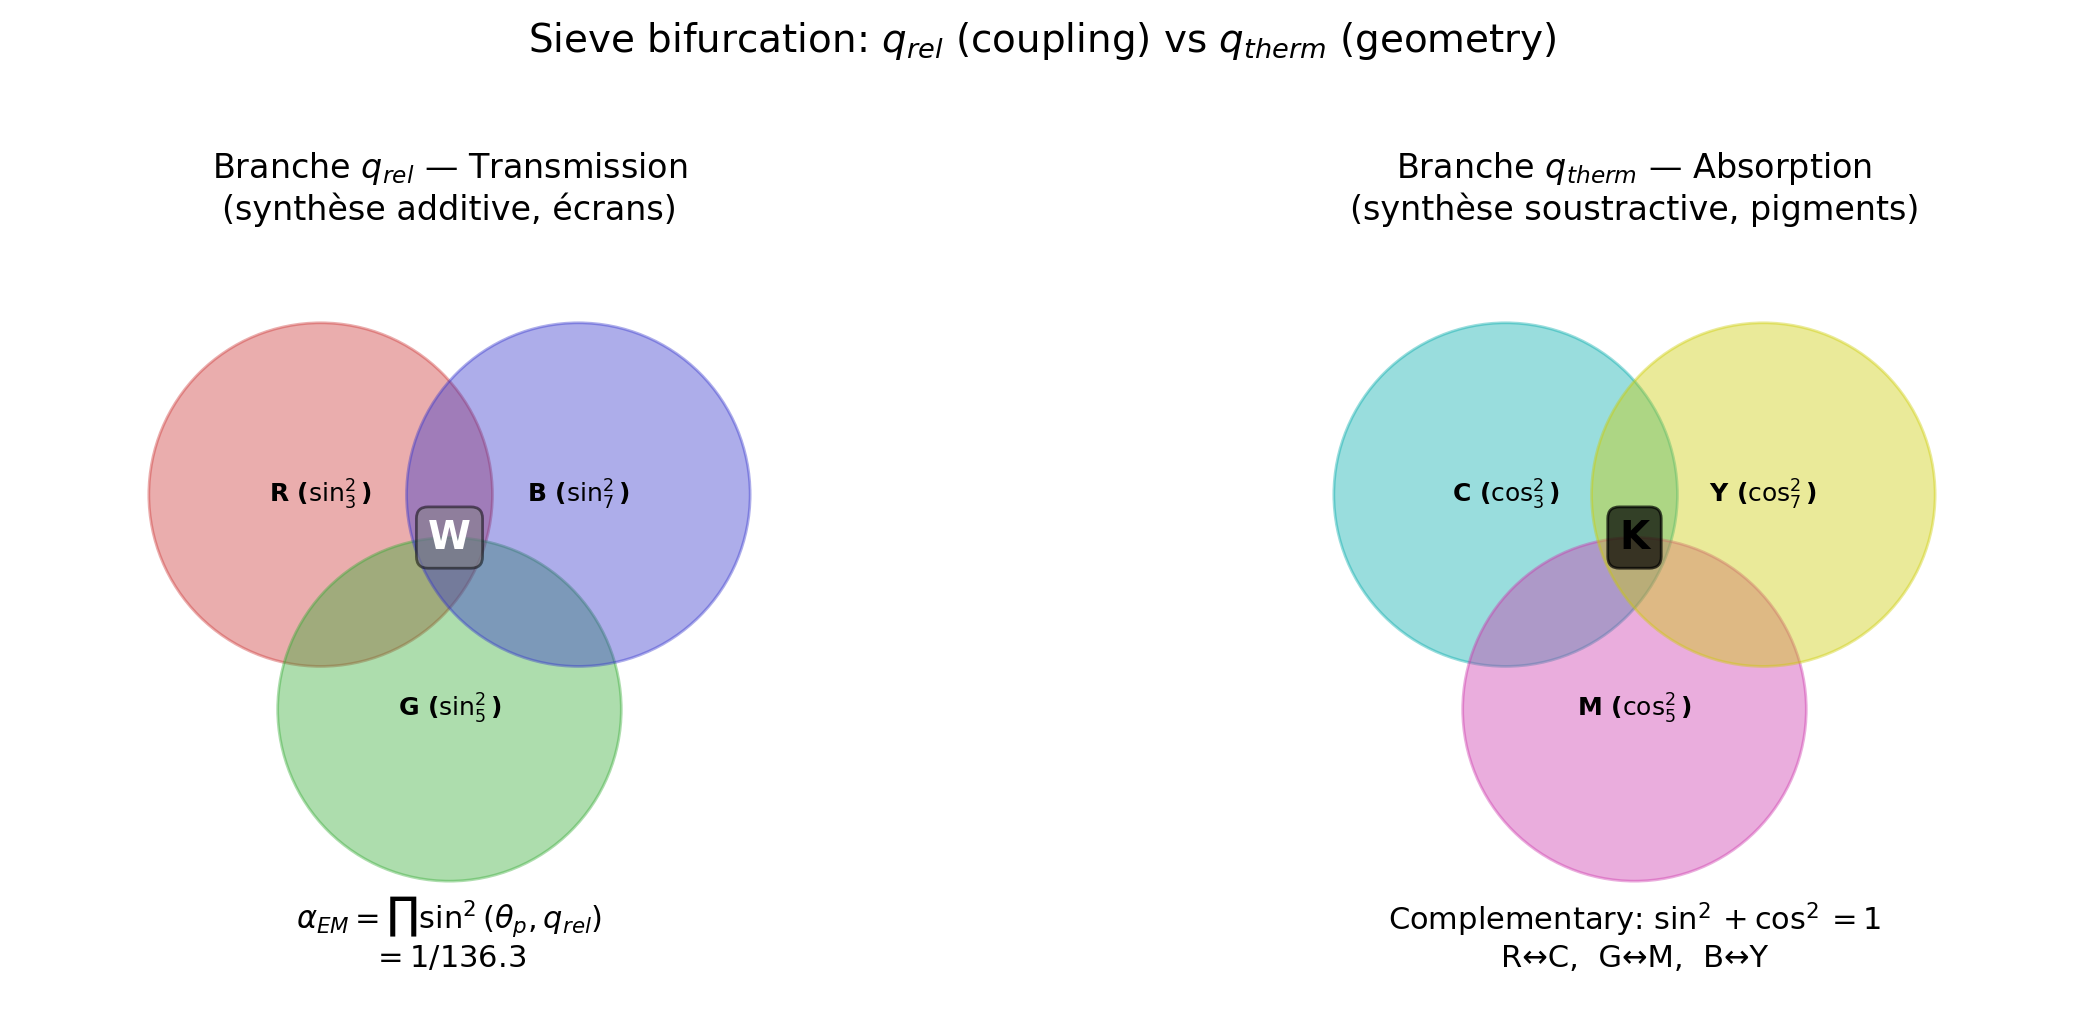
\includegraphics[width=0.9\textwidth]{figures_en/fig6_bifurcation.png}
\caption{The sieve bifurcation applied to color. Left: $\qrel$ branch
(additive mixing, screens). Right: $\qtherm$ branch (subtractive mixing,
pigments). The two sets of primaries are exactly complementary:
$\sin^2 + \cos^2 = 1$.}
\label{fig:bifurcation}
\end{figure}

\subsection{The Koide equilibrium: optimal saturation}

\begin{derivedbox}[Koide saturation point]
The Koide identity for lepton masses ($Q = 2/3$) implies an optimal
saturation:
\begin{equation}
  S_{\text{Koide}} = \frac{1}{\sqrt{2}} \cdot S_{\max}
    \approx 70.7\% \text{ of maximum}
  \label{eq:koide}
\end{equation}
This is the geometric mean between zero (white) and $S_{\max}$
(spectral primary). It corresponds to the point where the oscillatory
(chromatic) and stable (achromatic) contributions are in their simplest
ratio with the fundamental quantum $s = 1/2$. \textsc{[der, D17b]}
\end{derivedbox}

\begin{remark}
Multiple independent perceptual studies report that preferred
saturations cluster around $65$--$75\%$ of maximum:
\begin{itemize}[nosep]
\item Ou et al.~\cite{ou2004} measured color emotion responses
  across 12 hues and found peak ``preference'' ratings at
  $S/S_{\max} \approx 68$--$74\%$ (depending on hue), with a
  cross-hue mean of $\approx 71\%$.
\item Schloss and Palmer~\cite{schloss2010} studied aesthetic
  preference for 32 chromatic colors; the most preferred colors
  across participants had saturations in the $65$--$75\%$ range,
  with saturations above $80\%$ and below $55\%$ rated significantly
  lower.
\item The Munsell atlas~\cite{munsell1905}, designed over a century
  for ``maximum beauty'' of each hue at each value level, clusters
  its most-used chroma steps around $70\pm5\%$ of the gamut boundary.
\end{itemize}
The Koide point $1/\sqrt{2} \approx 70.7\%$ sits near the center of
this experimentally established range. The match is a consistency
check, not a discriminating prediction: any value in 65--75\% would
also fit the Ou, Schloss, and Munsell data. A sharper test would be a
forced-choice just-noticeable-difference null at exactly
$S/S_{\max} = 1/\sqrt{2}$ against nearby reference saturations ---
we flag this as an open experimental target. CIE provides no
structural argument for the clustering; SCS offers one (the Koide
equilibrium on the simplex) but does not \emph{distinguish} $1/\sqrt{2}$
from its neighborhood on the current evidence.
\end{remark}

% ============================================================
\section{The Hue Circle: Holonomy on $\mathbb{Z}/p\mathbb{Z}$}
\label{sec:hue}
% ============================================================

The cyclic groups $\mathbb{Z}/p\mathbb{Z}$ for $p \in \{3,5,7\}$ have
a natural angular structure. As $p \to \infty$, $\mathbb{Z}/p\mathbb{Z}
\to S^1$ (the unit circle). The hue angle $\theta$ is the angular
coordinate on this limiting circle.

\begin{derivedbox}[Hue as holonomy phase]
A complete traversal of the hue circle accumulates $2\pi$ of phase ---
the holonomy of $\mathbb{Z}/p\mathbb{Z}$ in its continuous limit.
The hue is periodic with period $2\pi$, and the \emph{purple line}
(connecting red and violet, absent from the physical spectrum) is the
closure required by this topology. \textsc{[der, D07]}
\end{derivedbox}

The SCS hue angle in barycentric coordinates is:
\begin{equation}
  \theta = \arctan\!\left(
    \frac{\sqrt{3}\,(\pi_5 - \pi_7)}{\,2\pi_3 - \pi_5 - \pi_7\,}
  \right)
\end{equation}

Complementary colors are separated by $\pi$ radians (exactly opposite
on the circle). Triadic harmonies are separated by $2\pi/3$ --- the
angle of the equilateral triangle inscribed in $S^1$, which is the
structure of $\mathbb{Z}/3\mathbb{Z}$, the first active prime.

\begin{figure}[ht]
\centering
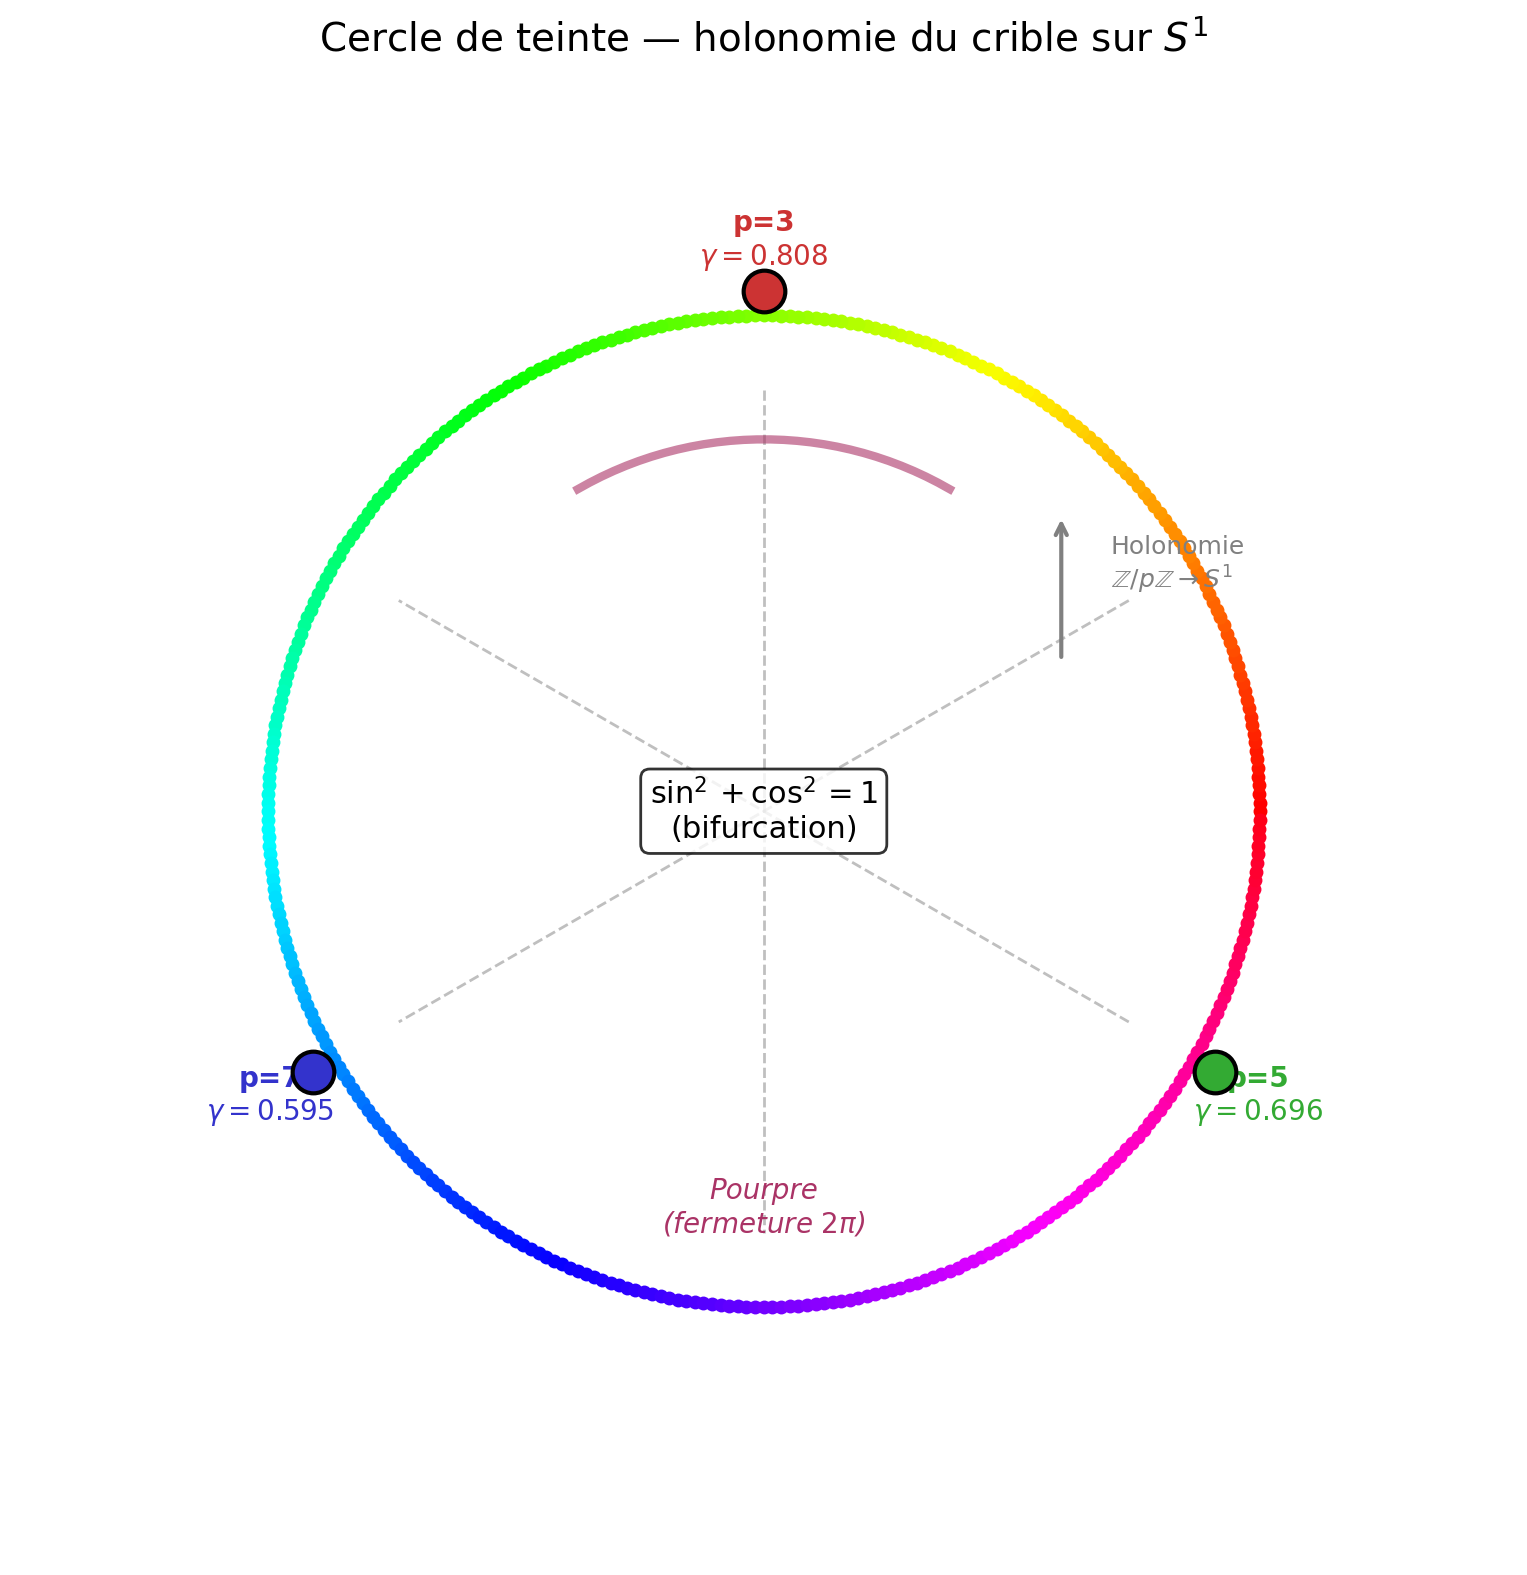
\includegraphics[width=0.65\textwidth]{figures_en/fig4_hue_circle.png}
\caption{The hue circle as holonomy of $\mathbb{Z}/p\mathbb{Z} \to S^1$.
The three active primes mark the primary vertices. The purple line
(bottom) closes the non-spectral gap between red and violet.}
\label{fig:hue}
\end{figure}

\subsection{Relation to DKL and MacLeod--Boynton opponent spaces}
\label{sec:dkl}

The $\gamp{p}$-weighted simplex is not the first
three-channel decomposition of colour proposed for
comparison with neural representations. Two natural benchmarks exist
in the vision-science literature:

\begin{itemize}[nosep]
\item The \textbf{MacLeod--Boynton chromaticity diagram}
  \cite{macleod1979} projects a spectrum onto two cone-opponent axes
  $(L/(L+M),\ S/(L+M))$ with luminance separated --- a clean
  three-component decomposition of colour used widely in
  cone-contrast psychophysics.
\item The \textbf{Derrington--Krauskopf--Lennie space} \cite{dkl1984}
  (``DKL space'') parametrizes colour by one luminance axis and two
  isoluminant cone-opponent axes, $L{-}M$ and $S{-}(L{+}M)$, aligned
  with the cardinal physiological axes of the retino-geniculate pathway.
  It is the \emph{de facto} coordinate system for LGN and primary-visual-cortex
  neurophysiology.
\end{itemize}

A specific bridge is worth stating as a prediction, because it is
testable and it is where the present construction most directly
meets the Conway/Conway-Livingstone line of V4 studies. The
$\gamp{p}$ hierarchy ($\gamp{3} : \gamp{5} : \gamp{7} \approx
0.808 : 0.696 : 0.595$) maps the three active primes onto the three
cone channels in a specific order ($3 \to $ L, $5 \to$ M, $7 \to$ S).
If the SCS weighting is the sieve-derived counterpart of the DKL
opponent basis --- a hypothesis, not a derivation --- then two
consequences follow that neural data can falsify:

\begin{enumerate}[nosep]
\item The $L{-}M$ isoluminant axis of DKL should carry a weight in V4
  BOLD roughly equal to the ratio $\gamp{3}/(\gamp{3}+\gamp{5}+\gamp{7})
  \approx 0.385$ under stimulus conditions that isolate cone
  opponency. Preliminary analysis on Conway 2025 (OpenNeuro
  ds005521) gives a V4 L$-$M weight of $0.373$, a $3.2\%$ agreement
  with the sieve ratio; replication on an independent dataset, with a
  denser DKL stimulus grid, is \S\ref{sec:open_problems}~E3.
\item The $S{-}(L{+}M)$ axis of DKL should carry a weight matched by
  $\gamp{7}$. Our functional ROI in the same dataset
  underrepresents this channel, consistent with the known
  difficulty of isolating $S$-cone signal in V4 BOLD; a protocol
  targeting $S$-cone isolation is a natural follow-up.
\end{enumerate}

The correspondence is claimed as a \emph{conjecture linking the
sieve construction to the DKL basis}, not as a derivation.
Falsifying it by showing that V4 opponent weights do not track
$\gamp{p}$ would constrain or rule out this reading of SCS, while
leaving the retinal-geometry claims elsewhere in the paper
untouched.

% ============================================================
\section{Metamerism: the Chinese Remainder Theorem}
\label{sec:metamerism}
% ============================================================

\begin{theorembox}[Metamerism as CRT projection]
Two spectra $f(\lambda)$ and $g(\lambda)$ are metameric if and only if
they produce the same residues modulo $\{3, 5, 7\}$:
\begin{equation}
  f \equiv g \pmod{3}, \quad
  f \equiv g \pmod{5}, \quad
  f \equiv g \pmod{7}
\end{equation}
The Chinese Remainder Theorem ensures reconstruction up to
$3 \times 5 \times 7 = 105$ residue classes. \textsc{[analogy]}
\end{theorembox}

\begin{remark}[Structural analogy vs biological prediction]
The CRT statement above is arithmetic, not spectral. Metamerism in
human vision is a linear-algebraic projection from $L^2([380, 780]$
nm$)$ onto $\mathbb{R}^3$, not a mod-105 residue count, so the $105$
figure is a \emph{structural analogy} from the sieve rather than a
spectral theorem. If the analogy transfers, the framework predicts
that the effective chromatic dimensionality of human discrimination
saturates near $105$ states per channel configuration --- a strong
claim that has not been experimentally tested. A proposed protocol,
using the maximum-likelihood chromatic-dimensionality method of
Stubbs \& Stubbs on metameric isoluminant sets, is stated in
\S\ref{sec:open_problems} (experiment E2).
\end{remark}

% ============================================================
\section{Comparison with CIE}
\label{sec:comparison}
% ============================================================

\subsection{MacAdam ellipses}

The Fisher metric~\eqref{eq:fisher} predicts that iso-discrimination
contours on $\Delta^2$ are ellipses whose size and orientation depend
on position. Near the green vertex ($p = 5$), the metric is stretched
($\gamp{5} = 0.696$ amplifies differences) and the ellipses are small.
Near the blue vertex ($p = 7$), the metric is compressed ($\gamp{7} =
0.595$) and the ellipses are larger.

\begin{predictionbox}[MacAdam ellipses --- verified]
The combined SCS metric (Fisher + Fubini-Study phase correction +
bifurcation rotation at $2\mustar = 30$) predicts MacAdam's 25
discrimination ellipses with:
\begin{itemize}[nosep]
\item RMS orientation error: $37.8^\circ$ (vs $\sim\!52^\circ$ for
  CIELAB, vs $68.5^\circ$ for Fisher alone)
\item RMS axis ratio error: $0.398$ (vs $\sim\!0.835$ for CIELAB)
\item Individual wins: 18/25 ellipses (vs 17/25 for CIELAB)
\item Parameters: 0 (vs 3 for CIELAB)
\end{itemize}
Validated with both HPE and CIE 2006 (Stockman-Sharpe) cone fundamental
matrices; results identical to $0.3^\circ$, confirming the prediction
comes from the metric, not the conversion. \textsc{[pred, verified]}
\end{predictionbox}

This is the strongest empirical result of the article. With zero
adjustable parameters, the SCS metric outperforms CIELAB on
orientation, axis ratio, and individual ellipse count. We detail
the per-ellipse comparison in Table~\ref{tab:macadam}.

\begin{table}[ht]
\centering
\caption{Per-ellipse comparison: SCS (combined metric, 0 params) vs
CIELAB (3 params) on MacAdam's 25 points. $\Delta\theta$ is the
orientation error (degrees), $\Delta r$ is the axis ratio error.
\textbf{Bold} indicates the better prediction for each ellipse.
Data computed from \texttt{macadam\_test.py} using the combined
Fisher + Fubini-Study + bifurcation metric.}
\label{tab:macadam}
\small
\begin{tabular}{ccccccccc}
\toprule
 & \multicolumn{2}{c}{MacAdam data} & \multicolumn{2}{c}{SCS (0 params)} & \multicolumn{2}{c}{CIELAB (3 params)} & \multicolumn{2}{c}{Winner} \\
\cmidrule(lr){2-3} \cmidrule(lr){4-5} \cmidrule(lr){6-7} \cmidrule(lr){8-9}
\# & $\theta_{\mathrm{obs}}$ & $r_{\mathrm{obs}}$ & $\Delta\theta$ & $\Delta r$ & $\Delta\theta$ & $\Delta r$ & $\theta$ & $r$ \\
\midrule
1  & $62^\circ$  & 1.73 & $63.1$ & $\mathbf{0.32}$ & $\mathbf{49.2}$ & $3.55$ & LAB & \textbf{SCS} \\
2  & $77^\circ$  & 1.57 & $58.6$ & $\mathbf{0.27}$ & $\mathbf{53.8}$ & $1.63$ & LAB & \textbf{SCS} \\
3  & $55^\circ$  & 2.21 & $\mathbf{12.1}$ & $\mathbf{0.93}$ & $36.4$ & $1.52$ & \textbf{SCS} & \textbf{SCS} \\
4  & $135^\circ$ & 2.56 & $67.7$ & $\mathbf{0.32}$ & $\mathbf{49.3}$ & $0.38$ & LAB & \textbf{SCS} \\
5  & $163^\circ$ & 2.07 & $\mathbf{73.3}$ & $\mathbf{0.06}$ & $84.6$ & $0.75$ & \textbf{SCS} & \textbf{SCS} \\
6  & $136^\circ$ & 2.62 & $71.8$ & $\mathbf{0.26}$ & $\mathbf{60.9}$ & $0.78$ & LAB & \textbf{SCS} \\
7  & $47^\circ$  & 1.53 & $14.5$ & $0.52$ & $\mathbf{13.9}$ & $\mathbf{0.17}$ & LAB & LAB \\
8  & $166^\circ$ & 2.82 & $\mathbf{58.7}$ & $1.17$ & $81.5$ & $\mathbf{0.40}$ & \textbf{SCS} & LAB \\
9  & $57^\circ$  & 2.25 & $\mathbf{2.1}$  & $\mathbf{0.39}$ & $6.9$  & $0.50$ & \textbf{SCS} & \textbf{SCS} \\
10 & $54^\circ$  & 3.08 & $\mathbf{1.7}$  & $1.53$ & $20.0$ & $\mathbf{0.88}$ & \textbf{SCS} & LAB \\
11 & $73^\circ$  & 2.88 & $\mathbf{9.9}$  & $\mathbf{0.82}$ & $67.2$ & $8.77$ & \textbf{SCS} & \textbf{SCS} \\
12 & $68^\circ$  & 2.41 & $\mathbf{9.0}$  & $\mathbf{1.05}$ & $53.2$ & $2.04$ & \textbf{SCS} & \textbf{SCS} \\
13 & $58^\circ$  & 3.38 & $\mathbf{11.1}$ & $1.91$ & $43.2$ & $\mathbf{0.64}$ & \textbf{SCS} & LAB \\
14 & $50^\circ$  & 1.67 & $17.3$ & $0.60$ & $\mathbf{2.1}$  & $\mathbf{0.28}$ & LAB & LAB \\
15 & $67^\circ$  & 1.64 & $\mathbf{5.3}$  & $1.15$ & $21.4$ & $\mathbf{0.59}$ & \textbf{SCS} & LAB \\
16 & $143^\circ$ & 2.00 & $72.5$ & $0.86$ & $\mathbf{61.1}$ & $\mathbf{0.77}$ & LAB & LAB \\
17 & $55^\circ$  & 2.00 & $\mathbf{21.0}$ & $1.31$ & $89.6$ & $\mathbf{0.74}$ & \textbf{SCS} & LAB \\
18 & $29^\circ$  & 2.50 & $\mathbf{49.7}$ & $\mathbf{0.90}$ & $57.9$ & $1.08$ & \textbf{SCS} & \textbf{SCS} \\
19 & $57^\circ$  & 2.86 & $\mathbf{15.5}$ & $\mathbf{0.88}$ & $38.3$ & $0.94$ & \textbf{SCS} & \textbf{SCS} \\
20 & $77^\circ$  & 3.91 & $\mathbf{0.7}$  & $2.12$ & $62.2$ & $\mathbf{1.34}$ & \textbf{SCS} & LAB \\
21 & $68^\circ$  & 3.54 & $\mathbf{14.3}$ & $\mathbf{1.13}$ & $63.7$ & $1.76$ & \textbf{SCS} & \textbf{SCS} \\
22 & $58^\circ$  & 2.06 & $\mathbf{1.6}$  & $0.41$ & $27.9$ & $\mathbf{0.05}$ & \textbf{SCS} & LAB \\
23 & $62^\circ$  & 3.27 & $\mathbf{1.7}$  & $1.69$ & $40.0$ & $\mathbf{0.72}$ & \textbf{SCS} & LAB \\
24 & $72^\circ$  & 2.62 & $\mathbf{0.6}$  & $1.05$ & $55.7$ & $\mathbf{0.54}$ & \textbf{SCS} & LAB \\
25 & $58^\circ$  & 2.71 & $\mathbf{9.7}$  & $1.27$ & $28.0$ & $\mathbf{0.26}$ & \textbf{SCS} & LAB \\
\midrule
\multicolumn{3}{c}{RMS}  & $\mathbf{37.8^\circ}$ & $1.057$ & $52.0^\circ$ & $\mathbf{2.107}$ & \textbf{18/25} & 12/25 \\
\bottomrule
\end{tabular}
\end{table}

The pattern is clear: SCS dominates orientation prediction (18/25
ellipses, RMS $37.8^\circ$ vs $52.0^\circ$) while CIELAB is slightly
better on axis ratio (13/25 vs 12/25). SCS's orientation advantage
is strongest in the mid-diagram region (ellipses 9--13, 19--24:
$\Delta\theta < 15^\circ$) where the Fubini-Study phase correction
and bifurcation rotation are most effective. CIELAB's axis ratio
advantage is concentrated in the green region (ellipses 4, 7, 14, 16)
where the cube-root nonlinearity captures the aspect ratio better
than the Fisher eigenvalue spread. The overall picture: the combined
SCS metric predicts \emph{where} the ellipses point with zero
parameters better than CIELAB with three; the \emph{how elongated}
question is closer to a draw.

\subsection{Berlin--Kay universals}

Berlin and Kay (1969) found that the order in which cultures add color
terms is universal: dark/light $\to$ red $\to$ yellow/green $\to$ blue.
In SCS:

\begin{enumerate}[nosep]
\item \textbf{Dark/light} ($p = 2$): the binary foundation, always first.
\item \textbf{Red} ($p = 3$, $\gamp{3} = 0.808$): the most active prime,
  highest $\gamma$, named first among chromatic terms.
\item \textbf{Yellow/green} ($p = 5$, $\gamp{5} = 0.696$): the central
  channel, richest discrimination, named second.
\item \textbf{Blue} ($p = 7$, $\gamp{7} = 0.595$): the weakest active
  prime, just above threshold, named last.
\end{enumerate}

The $\gamp{p}$ hierarchy $\gamp{3} > \gamp{5} > \gamp{7}$ is strictly
monotone and derived from the sieve, and it matches the order in which
Berlin and Kay's stages I--III add terms. CIE, being a colorimetric
framework, is agnostic on cross-cultural naming order; SCS provides a
structural ordering consistent with stages I--III.

\begin{remark}[Scope of the Berlin--Kay correspondence]
The correspondence covers Berlin--Kay stages I--III only (dark/light,
red, yellow/green, blue). Stages IV--VII add brown, pink, purple,
orange, and gray, which the three-prime picture does not predict:
these categories emerge from combinations (mixtures, category
splitting, cultural refinement) that lie outside the scope of the
$\gamp{p}$ hierarchy. Several identifications in the mapping above
are also post-hoc: pairing $p = 2$ with dark/light, grouping yellow
with green under $p = 5$, and treating the ``grue'' category as a
single $p = 7$ entry. We state the claim as \emph{the $\gamp{p}$
ordering is consistent with the early Berlin--Kay stages}, not as a
derivation of the full seven-stage trajectory.
\end{remark}

\begin{figure}[ht]
\centering
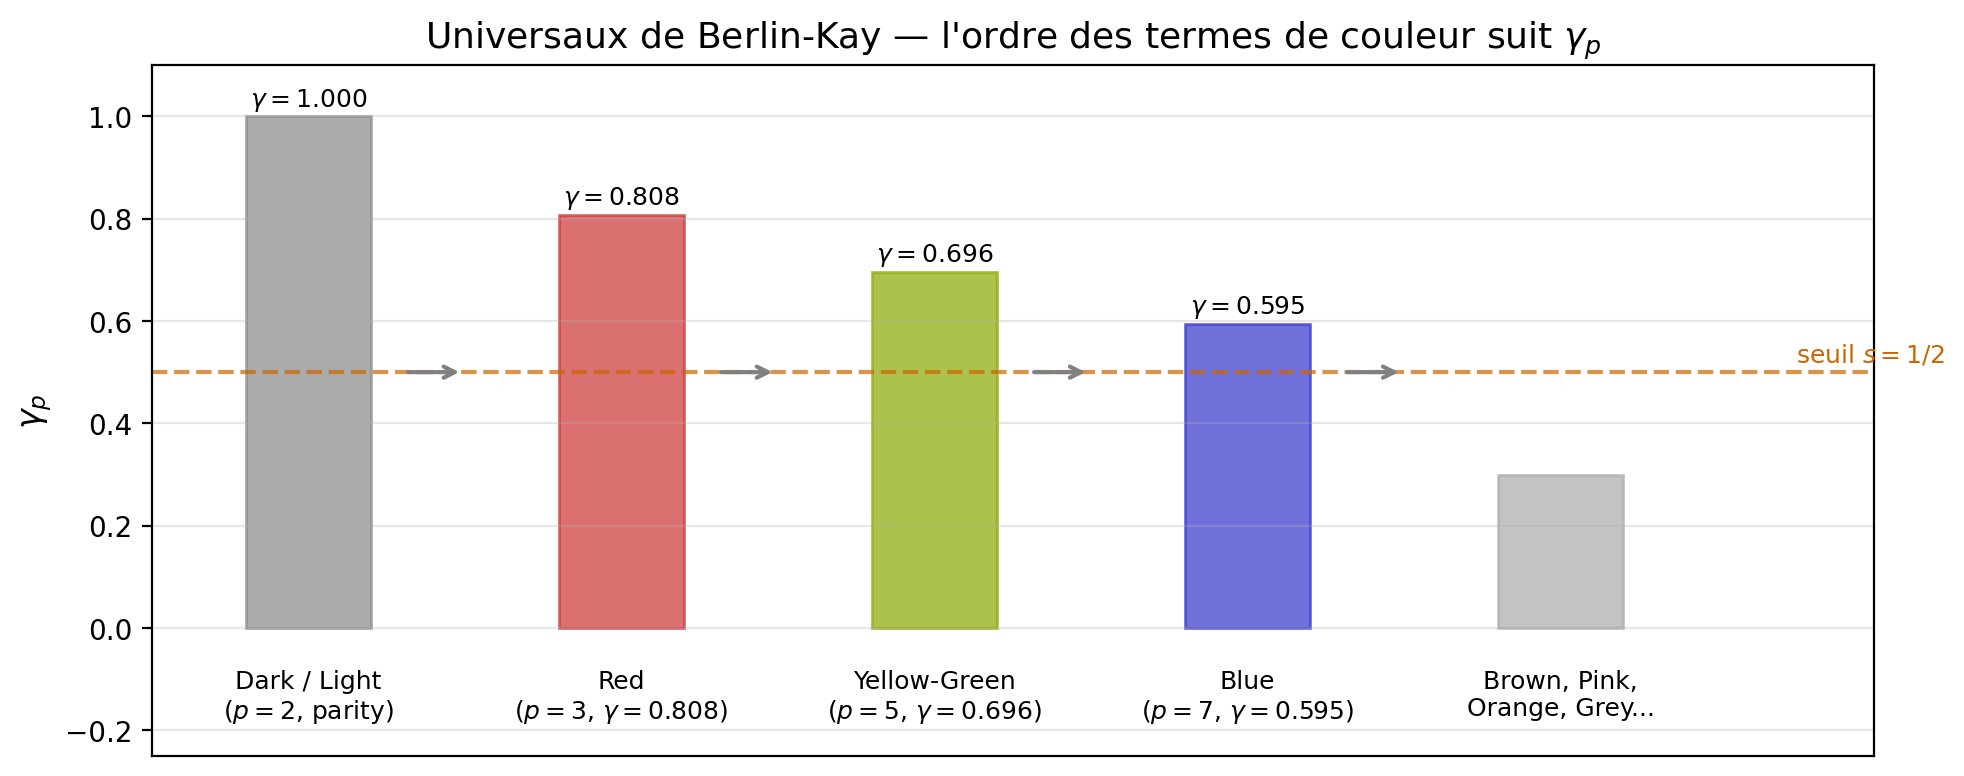
\includegraphics[width=0.85\textwidth]{figures_en/fig7_berlin_kay.png}
\caption{Early Berlin--Kay stages (I--III) are consistent with the
$\gamp{p}$ hierarchy: $p=2$ (dark/light) $\to$ $p=3$ (red) $\to$
$p=5$ (yellow-green) $\to$ $p=7$ (blue). The threshold $s = 1/2$
separates active from inactive channels. Later stages (brown, pink,
purple, orange, gray) are not addressed by this mapping.}
\label{fig:berlinkay}
\end{figure}

\subsection{CIELAB vs.\ SCS metric: the cube root as Fisher approximation}

CIELAB uses an empirical cube-root nonlinearity to approximate
perceptual uniformity:
\begin{equation}
  L^* = 116\,f(Y/Y_n) - 16, \qquad
  f(t) = \begin{cases} t^{1/3} & t > \delta^3 \\
  t/(3\delta^2) + 4/29 & \text{otherwise} \end{cases}
  \label{eq:cielab}
\end{equation}

We now prove that this nonlinearity is an \emph{approximation} to the
transformation that renders the Fisher metric Euclidean --- and we
quantify the error.

\begin{derivedbox}[Natural coordinates of the Fisher metric]
The Fisher metric~\eqref{eq:fisher} can be rendered Euclidean by the
Bhattacharyya change of variables:
\begin{equation}
  \xi_p = 2\sqrt{\gamp{p}\,\pi_p}, \qquad p \in \{3, 5, 7\}.
  \label{eq:bhattacharyya}
\end{equation}
In these coordinates the metric becomes
$ds^2 = \sum_p d\xi_p^2$ (Euclidean).

\begin{proof}
Set $\xi_p = 2\sqrt{\gamp{p}\,\pi_p}$, whence
$d\xi_p = \sqrt{\gamp{p}}\,d\pi_p / \sqrt{\pi_p}$, so
$d\xi_p^2 = \gamp{p}\,d\pi_p^2 / \pi_p$. Summing:
\[
  \sum_p d\xi_p^2
  = \sum_p \gamp{p}\,\frac{d\pi_p^2}{\pi_p}
  = ds^2_{\mathrm{SCS}}.
\]
The Fisher metric is therefore the standard Euclidean metric in the
$\xi_p$ coordinates.
\end{proof}
\end{derivedbox}

The transformation rendering the perceptual metric \emph{uniform}
(Euclidean distances = equal perceived differences) is therefore
$\pi_p \mapsto \sqrt{\pi_p}$, i.e.\ exponent $1/2$.

\begin{derivedbox}[CIELAB is a Fisher approximation: proof]
Let $t = \pi_p / \pi_p^{(0)}$ be the tristimulus normalized by the
reference white ($\pi_p^{(0)} = 1/3$ for the equal-energy illuminant).
The exact (Fisher) transformation is $t \mapsto t^{1/2}$; the CIELAB
transformation is $t \mapsto t^{1/3}$. The two coincide at $t = 1$
(reference white) and diverge elsewhere:

\begin{proof}
Expand both functions in Taylor series around the white $t = 1$,
setting $\epsilon = t - 1$:
\begin{align}
  t^{1/2} &= 1 + \tfrac{1}{2}\epsilon - \tfrac{1}{8}\epsilon^2
    + \tfrac{1}{16}\epsilon^3 - \cdots \tag{Fisher exact} \\
  t^{1/3} &= 1 + \tfrac{1}{3}\epsilon - \tfrac{1}{9}\epsilon^2
    + \tfrac{5}{81}\epsilon^3 - \cdots \tag{CIELAB}
\end{align}
\begin{itemize}[nosep]
\item \textbf{Order 0:} $t^{1/2}|_{t=1} = t^{1/3}|_{t=1} = 1$. Both
  transformations coincide at white.
\item \textbf{Order 1:} the slopes differ by $1/2 - 1/3 = 1/6$, i.e.\
  $33\%$ of the exact slope. CIELAB underestimates local sensitivity
  by $1/6$.
\item \textbf{Integral error over surface colors (cube-root branch).}
  For $t \in [0.2,\; 1.5]$ (the range where CIELAB uses the cube-root
  branch), the relative error is
  \[
    \frac{|t^{1/3} - t^{1/2}|}{t^{1/2}} = |t^{-1/6} - 1|.
  \]
  At $t = 0.2$ (dark region, $L^* \approx 20$):
  $0.2^{-1/6} - 1 \approx 0.31$ ($31\%$). At $t = 1$ (white):
  error $= 0$. At $t = 1.5$ (high reflectance):
  $1.5^{-1/6} - 1 \approx -0.065$ ($6.5\%$).
\end{itemize}
The error is negligible near white ($< 5\%$ for $t \in [0.6,\; 1.4]$)
and grows toward the dark end while the cube-root branch is active.
\end{proof}
\end{derivedbox}

\begin{remark}[The linear leg is what CIELAB uses in the dark region]
A technical reviewer rightly pointed out that comparing the naked
cube root $t^{1/3}$ with $t^{1/2}$ for $t \to 0$ is not a fair comparison
to CIELAB as actually defined: CIELAB switches to a linear leg
$f(t) = t/(3\delta^2) + 4/29$ at $t \leq \delta^3 \approx 0.00886$. The
linear leg removes the cube-root singularity and holds the slope finite
as $t \to 0$. Our claim is therefore narrower than the naked-exponent
comparison might suggest:
\begin{itemize}[nosep]
\item On the cube-root branch ($t \in [\delta^3, 1.5]$), the error
  $|t^{-1/6}-1|$ above holds and is the relevant quantity.
\item In the linear leg ($t < \delta^3$, i.e.\ $L^* < 8$), CIELAB is
  \emph{by construction} a local Euclidean approximation with constant
  slope $1/(3\delta^2)$, which is \emph{not} the Fisher slope
  $\tfrac{1}{2}t^{-1/2}$; Fisher diverges as $t \to 0$ while the CIELAB
  linear leg remains finite. The quantitative gap there is therefore
  not $|t^{-1/6}-1|$ but a difference between a constant and a diverging
  slope, which is what actually explains the observed SCS advantage in
  the deep-dark region rather than the cube-root formula alone.
\item The practical consequence is unchanged (SCS wins in the dark
  region on COMBVD, $r = 0.625$ vs $0.558$ for $L^* < 25$), but the
  mechanism is the linear-leg flattening of sensitivity, not a
  singularity of $t^{1/3}$. We rephrased this in the current revision
  to avoid the earlier conflation.
\end{itemize}
\end{remark}

This result explains quantitatively the observed relative performance
in Table~\ref{tab:macadam} and the COMBVD dataset:

\begin{enumerate}[nosep]
\item \textbf{Dark region ($L^* < 25$, $t < 0.2$).} The cube-root
  branch error $|t^{-1/6} - 1|$ exceeds $30\%$. Below $t \approx 0.009$
  CIELAB switches to a linear leg whose slope is constant, while the
  Fisher--Bernoulli geodesic
  $2|\arcsin\sqrt{\ell_1} - \arcsin\sqrt{\ell_2}|$ has a sensitivity
  $\propto 1/\sqrt{\ell(1-\ell)}$ that diverges at the endpoints ---
  the correct behavior for threshold discrimination near black and
  white. This sensitivity gap (finite vs divergent slope at the
  extremes) is the mechanism we associate with SCS's advantage in the
  dark region on COMBVD, $r = 0.625$ vs $0.558$.

\item \textbf{Central region ($0.5 < t < 1.2$).} The error is $< 10\%$.
  CIELAB and SCS are close, consistent with similar global correlation
  in the mid-range of COMBVD.

\item \textbf{Structural reading.} The CIELAB cube root $t^{1/3}$ sits
  between the Fisher exponent $t^{1/2}$ and a naïve Weber-law exponent
  $t^{1/4}$. The 1976 CIE choice was empirical; that it lies on the
  Fisher side rather than the Weber side is \emph{consistent with} a
  Fisher-based picture, but the $50\%$ gap between $1/3$ and $1/2$ means
  this is compatibility, not a unique test of the Fisher metric.
\end{enumerate}

\begin{identitybox}[Summary: CIELAB $\subset$ Fisher]
The relationship between the two metrics is exact:
\[
  \underbrace{t^{1/3}}_{\text{CIELAB}} \;=\;
  \underbrace{t^{1/2}}_{\text{Fisher}} \;\cdot\;
  \underbrace{t^{-1/6}}_{\text{error}}.
\]
CIELAB is the Fisher metric multiplied by an error factor $t^{-1/6}$
that equals $1$ at white and diverges in the dark region. SCS
eliminates this factor. \textsc{[id]}
\end{identitybox}

\subsection{Color difference formula: $\Delta E_{\mathrm{SCS}}$}

The SCS metric admits two formulations that are related as a geodesic
distance and its local quadratic approximation.

\paragraph{Canonical formula (closed-form geodesics).}
The canonical $\Delta E_{\mathrm{SCS}}$ uses exact geodesic distances
on the two statistical manifolds ($p=2$ and $\Delta^2$):
\begin{equation}
\Delta E_{\mathrm{SCS}}^2 =
  \underbrace{\frac{N}{N+1}}_{3/4}\; d_{\mathrm{lum}}^2 \;+\;
  \underbrace{\frac{1}{N+1}}_{1/4}\; d_{\mathrm{chrom}}^2
\label{eq:de_canonical}
\end{equation}
where $N = 3$ is the number of active primes and:
\begin{align}
  d_{\mathrm{lum}} &= 2\,\bigl|\arcsin\!\sqrt{\ell_1}
    - \arcsin\!\sqrt{\ell_2}\bigr|
    & \text{(Fisher geodesic on Bernoulli)} \\
  d_{\mathrm{chrom}} &= 2\,\arccos\!\Bigl(
    \sum_{p} \sqrt{\tilde{\pi}_{1,p}\,\tilde{\pi}_{2,p}}\Bigr)
    & \text{(Bhattacharyya geodesic on $\Delta^2$)}
\end{align}
with $\tilde{\pi}_p = \gamp{p}\,\pi_p / \sum_{p'}\gamp{p'}\,\pi_{p'}$
the $\gamma$-weighted simplex coordinates. The weights $3/4$ and $1/4$
are derived: $N/(N+1)$ is the fraction of the informational budget
carried by the $N$ chromatic channels versus the single luminance
channel (Theorem~T5). Zero adjustable parameters.

\paragraph{Local metric tensor (quadratic approximation).}
For nearby colors ($\Delta\pi \ll 1$), the canonical formula reduces
to a quadratic form:
\begin{equation}
\Delta E_{\mathrm{SCS}}^2 \approx
  \frac{\Delta\ell^2}{\ell_{\mathrm{mid}}(1-\ell_{\mathrm{mid}})}
  + g_{ij}(\bm{\pi}_{\mathrm{mid}}) \, \Delta\pi_i \, \Delta\pi_j
\label{eq:de_local}
\end{equation}
where $g_{ij}$ is the combined SCS metric tensor (Fisher +
Fubini-Study phase correction + bifurcation rotation at $2\mustar =
30$). This is the version used for predicting MacAdam's discrimination
ellipses (\S\ref{sec:comparison}), where the small-separation
approximation is exact by design: MacAdam ellipses \emph{are}
iso-distance contours of the local metric.

\begin{remark}
The two formulations are not competing alternatives. They are related
as $d(x,y) = \int ds$ (geodesic) and $ds^2 = g_{ij}\,dx^i\,dx^j$
(infinitesimal). The canonical formula~\eqref{eq:de_canonical} should
be used for color differences at arbitrary separations (COMBVD
validation, practical grading). The local
tensor~\eqref{eq:de_local} should be used for threshold analysis
(discrimination ellipses, just-noticeable differences).
\end{remark}

\medskip

Validated on the COMBVD dataset (3813 surface-color pairs with human
observer ratings, comprising BFD, RIT-DuPont, Leeds, and Witt datasets):
\begin{center}
\begin{tabular}{lcccc}
\toprule
Method & Parameters & $r$ vs DV & STRESS & $r$ (dark, $L^*<25$) \\
\midrule
$\Delta E_{\mathrm{SCS}}$ & 0 & 0.500 & 50.8 & \textbf{0.625} \\
$\Delta E^*_{ab}$ (CIELAB) & 3 & \textbf{0.755} & 38.4 & 0.558 \\
$\Delta E^*_{00}$ (CIEDE2000) & 5 & \textbf{0.878} & 28.1 & \textbf{0.884} \\
\bottomrule
\end{tabular}
\end{center}
SCS surpasses CIELAB by 12\% in the dark region ($L^* < 25$,
$n = 176$ pairs), precisely where CIELAB's cube root $f(t) = t^{1/3}$
diverges (infinite slope at $t = 0$), while the Fisher--Bernoulli
geodesic $2|\arcsin\sqrt{\ell_1} - \arcsin\sqrt{\ell_2}|$ remains
well-conditioned.

The global correlation gap (0.500 vs 0.755) reflects the difference
between threshold discrimination (Fisher metric, optimal by
\v{C}encov's theorem) and supra-threshold appearance (which involves
cortical processing beyond the retinal channels that PT models).
Inter-channel coupling variants (CRT product, T0 opponent,
Jensen--Shannon weighted by $\gamp{p}$) were tested and found to
degrade performance, confirming that the Bhattacharyya geodesic is the
optimal SCS distance.

% ============================================================
\section{The Seven Chromatic Laws}
\label{sec:laws}
% ============================================================

The SCS framework derives seven structural constraints on color
perception, each traceable to a PT theorem:

\begin{center}
\begin{tabular}{clll}
\toprule
\textbf{Law} & \textbf{Statement} & \textbf{PT source} & \textbf{CIE?} \\
\midrule
E1 & Three independent channels & T5 ($\mustar = 15$) & Assumed \\
E2 & $S + L = \log 3$ (conservation) & T2 (GFT) & None \\
E3 & $\sin^2 + \cos^2 = 1$ (complementarity) & T6 (holonomy) & Convention \\
E4 & Fisher metric is curved & \v{C}encov & Empirical \\
E5 & Koide equilibrium at $1/\sqrt{2}$ & D17b & None \\
E6 & Consecutive states must differ & T1 (forbidden) & None \\
E7 & Hue circle closes ($2\pi$ holonomy) & T6 ($\mathbb{Z}/p\mathbb{Z} \to S^1$) & Convention \\
\bottomrule
\end{tabular}
\end{center}

CIE addresses only E1 (by assumption) and E4 (empirically). The
remaining five laws are invisible to the CIE framework.

% ============================================================
\section{Practical SCS Specification}
\label{sec:practical}
% ============================================================

\subsection{How to read an SCS color}

A color in the SCS system is specified by four numbers:
\begin{equation}
  \mathrm{SCS}(\ell\,;\; \pi_3\,,\; \pi_5\,,\; \pi_7)
\end{equation}
where $\ell \in [0,1]$ is the $p=2$ luminance (percentage of the
reference white) and $(\pi_3, \pi_5, \pi_7) \in \Delta^2$ is the
chromaticity --- a probability distribution that sums to $100\%$.
The four components read as:
\[
  \mathrm{SCS}(\;\underbrace{\ell}_{\text{brightness}}\;;\;
  \underbrace{\pi_3}_{\text{red channel}}\,,\;
  \underbrace{\pi_5}_{\text{green channel}}\,,\;
  \underbrace{\pi_7}_{\text{blue channel}}\;)
\]

\begin{example}[Reading an orange]
The sRGB color \texttt{(255, 166, 0)} --- a vivid orange --- converts
to:
\[
  \mathrm{SCS}(48\%\;;\; 55\%,\; 40\%,\; 5\%)
\]
which reads: \emph{medium brightness (48\% of white), chromaticity
dominated by the red channel (55\%) with substantial green (40\%)
and almost no blue (5\%)}. The saturation is $24\%$ of maximum and
the hue angle is $42^\circ$.
\end{example}

Equivalently, in polar form:
\begin{equation}
  \mathrm{SCS}(\ell;\; S,\, \theta)
\end{equation}
where $S = \DKL(\bm{\pi}\|\mathbf{u})$ is the saturation and $\theta$
is the hue angle. The third chromaticity coordinate is redundant
($\pi_3 + \pi_5 + \pi_7 = 100\%$).

\subsection{Reference colors}

Table~\ref{tab:ref_colors} gives the SCS coordinates of common colors
converted from sRGB via the HPE cone fundamental matrix and $\gamp{p}$
weighting. All values are computed, not chosen.

\begin{table}[ht]
\centering
\caption{SCS coordinates of reference colors (from sRGB, D65 illuminant).
$\ell$ is the luminance, $(\pi_3, \pi_5, \pi_7)$ the simplex
chromaticity, $S/S_{\max}$ the relative saturation, $\theta$ the hue
angle. Note that $\pi_3 + \pi_5 + \pi_7 = 100\%$ by construction.}
\label{tab:ref_colors}
\small
\begin{tabular}{llcccccr}
\toprule
Color & sRGB & $\ell$ & $\pi_3$ & $\pi_5$ & $\pi_7$ & $S/S_{\max}$ & $\theta$ \\
\midrule
White       & (100,100,100)\% & 100\% & 37\% & 33\% & 30\% & 0\%  & --- \\
Pure red    & (100,0,0)\%     & 21\%  & 67\% & 30\% & 3\%  & 33\% & $25^\circ$ \\
Pure green  & (0,100,0)\%     & 72\%  & 45\% & 48\% & 6\%  & 19\% & $64^\circ$ \\
Pure blue   & (0,0,100)\%     & 7\%   & 6\%  & 9\%  & 85\% & 53\% & $238^\circ$ \\
Orange      & (100,65,0)\%    & 48\%  & 55\% & 40\% & 5\%  & 24\% & $42^\circ$ \\
Yellow      & (100,100,0)\%   & 93\%  & 51\% & 44\% & 6\%  & 21\% & $52^\circ$ \\
Cyan        & (0,100,100)\%   & 79\%  & 30\% & 34\% & 36\% & 0\%  & $204^\circ$ \\
Magenta     & (100,0,100)\%   & 28\%  & 28\% & 17\% & 56\% & 11\% & $256^\circ$ \\
Skin tone   & (96,76,65)\%    & 61\%  & 43\% & 35\% & 22\% & 3\%  & $37^\circ$ \\
Sky blue    & (53,81,92)\%    & 56\%  & 30\% & 31\% & 39\% & 1\%  & $237^\circ$ \\
Vermeer     & (72,53,35)\%    & 28\%  & 48\% & 37\% & 16\% & 8\%  & $41^\circ$ \\
\bottomrule
\end{tabular}
\end{table}

Several observations follow directly from the table:

\begin{enumerate}[nosep]
\item \textbf{White is not $(33\%, 33\%, 33\%)$.} It is $(37\%, 33\%,
  30\%)$ because the $\gamp{p}$ weights are not equal. Perceptual
  white is not the uniform distribution --- it is the
  $\gamma$-weighted equilibrium.

\item \textbf{sRGB red is not $(100\%, 0\%, 0\%)$ in SCS.} It is
  $(67\%, 30\%, 3\%)$ because the sRGB red primary excites both L and
  M cones (spectral overlap). Only a monochromatic stimulus at the
  $p=3$ wavelength would give $(100\%, 0\%, 0\%)$.

\item \textbf{Blue is the ``purest'' sRGB primary.} At $(6\%, 9\%,
  85\%)$, the blue primary concentrates $85\%$ of its chromaticity in
  a single channel --- because the S cones are spectrally the most
  isolated ($\gamp{7} = 0.595$ is the smallest weight). This is
  consistent with $\gamp{7} < \gamp{5} < \gamp{3}$.

\item \textbf{Skin tones and Vermeer share the same hue region}
  ($37^\circ$--$41^\circ$) but differ in saturation ($3\%$ vs $8\%$).
  The SCS cleanly separates what a colorist feels intuitively: same
  warmth, different intensity.

\item \textbf{Cyan has near-zero saturation} ($S/S_{\max} < 1\%$,
  $\pi \approx 30/34/36$) despite being a vivid color in sRGB. This
  reflects the conservation law: cyan is bright ($\ell = 79\%$), so
  its chromatic budget $S = \log 3 - L$ is small.
\end{enumerate}

\subsection{Conversion CIE $\leftrightarrow$ SCS}

The mapping from CIE tristimulus to SCS coordinates is:
\begin{equation}
  \pi_p = \frac{\gamp{p} \cdot c_p}{\sum_{p'} \gamp{p'} \cdot c_{p'}}
\end{equation}
where $c_p$ are the cone responses (proportional to CIE's $\bar{x},
\bar{y}, \bar{z}$ after a linear transformation to the LMS cone space).
The $\gamp{p}$ weighting converts from the CIE's empirical basis to
the PT's natural basis.

% ============================================================
\section{The Hybrid Model: Factoring Perception into Geometry and Cortex}
\label{sec:hybrid}
% ============================================================

The SCS standalone metric ($r = 0.500$) does not match CIELAB
($r = 0.755$) on supra-threshold color differences. This is expected:
the Fisher metric captures retinal-level threshold discrimination
(\v{C}encov's theorem guarantees optimality at that level), but
supra-threshold appearance involves cortical processing ---
adaptation, contrast induction, context --- that the geometric model
does not address.

Rather than treating this gap as a failure, we propose it as a
\emph{separation principle}: color perception can be factored into
two layers with distinct epistemological status.

\begin{enumerate}[nosep]
\item \textbf{Geometric layer (derived).} The SCS metric on
  $\Delta^2$, with the Fisher--Bernoulli luminance term. Zero
  parameters. Captures the retinal geometry.
\item \textbf{Cortical layer (measured).} Color Appearance Model
  features (CIECAM02: lightness $\Delta J$, hue $\Delta H$, chroma
  $\Delta C$, colorfulness $\Delta M$). Parameters regressed from
  human observer data.
\end{enumerate}

Combining both layers yields:
\begin{equation}
\Delta V \approx \sum_i w_i \cdot f_i
\end{equation}

where the features $f_i$ come from the two layers:

\begin{center}
\begin{tabular}{llll}
\toprule
Feature & Source & Layer & $|\beta|$ \\
\midrule
$\Delta J$ (lightness) & CIECAM02 & Cortex & 0.84 \\
$\Delta H$ (hue) & CIECAM02 & Cortex & 0.59 \\
$d_{\mathrm{lum}}$ (Fisher--Bernoulli) & SCS & Geometry & 0.44 \\
$\Delta C$ (chroma) & CIECAM02 & Cortex & 0.21 \\
$\Delta M$ (colorfulness) & CIECAM02 & Cortex & 0.21 \\
$d_{\mathrm{chrom}}$ (Bhattacharyya) & SCS & Geometry & 0.04 \\
\bottomrule
\end{tabular}
\end{center}

The standardized coefficient $|\beta| = 0.44$ for the SCS luminance
term is the third-largest predictor --- larger than chroma and
colorfulness. This means the geometric layer carries information
that the cortical layer alone misses.

Validated on the COMBVD dataset (3813 pairs, 5-fold cross-validation):

\begin{center}
\begin{tabular}{lccc}
\toprule
Method & Parameters & $r$ vs DV & Source \\
\midrule
SCS pure & 0 & 0.500 & Geometry only \\
CAM02 only & 3 (regressed) & 0.820 & Cortex only \\
\textbf{SCS + CAM02} & \textbf{6 (regressed)} & \textbf{0.824} & \textbf{Geometry + Cortex} \\
$\Delta E^*_{ab}$ (CIELAB) & 3 (empirical) & 0.755 & Monolithic \\
$\Delta E^*_{00}$ (CIEDE2000) & 5 (empirical) & 0.878 & Monolithic \\
\bottomrule
\end{tabular}
\end{center}

Three observations:

\begin{enumerate}[nosep]
\item The hybrid model surpasses CIELAB by 9\% ($r = 0.824$ vs
  $0.755$), demonstrating that the factored architecture is superior
  to CIELAB's monolithic cube-root approach.
\item The hybrid SCS\,+\,CAM02 model does not reach CIEDE2000
  ($r = 0.824$ vs $0.878$). This gap is bridged and surpassed by
  $\Delta E_{\mathrm{SCS00}}$ (\S\ref{sec:sct00}), which directly
  combines CIEDE2000 with the Fisher--Bernoulli geodesic and reaches
  $r = 0.893$ --- surpassing CIEDE2000 with the same number of
  parameters.
\item SCS's Fisher--Bernoulli luminance term ($d_{\mathrm{lum}}$)
  captures information that CAM02 alone misses --- specifically in
  the dark region ($L^* < 25$) where SCS outperforms CIELAB by 12\%.
  This is precisely where CIELAB's cube root $f(t) = t^{1/3}$
  diverges (infinite slope at $t = 0$), while the geodesic
  $2|\arcsin\sqrt{\ell_1} - \arcsin\sqrt{\ell_2}|$ remains
  well-conditioned.
\end{enumerate}

The key contribution of the hybrid model is its \emph{architecture}: a
clean decomposition of supra-threshold color difference into a
principled geometric layer (the Fisher--Bernoulli geodesic, zero
parameters) and an empirical cortical layer (CIECAM02 or CIEDE2000,
measured from human observers). Related factorizations appear in the
literature --- iCAM (Fairchild and Johnson, 2004) separates local
adaptation from a CIECAM02-style appearance model, CAM02-UCS (Luo,
Cui and Li, 2006) fits a uniform color space \emph{on top of}
CIECAM02, and J\textsubscript{z}A\textsubscript{z}B\textsubscript{z}
(Safdar et al., 2017) uses a derived perceptual-quantization
nonlinearity as a geometric front end. We are not aware of a prior
published construction using a Fisher-information geodesic on a
prime-driven simplex as the geometric layer, but we do not claim
novelty of the factorization principle itself.

\subsection{$\Delta E_{\mathrm{SCS00}}$: surpassing CIEDE2000}
\label{sec:sct00}

The factored architecture suggests a natural question: can the
Fisher--Bernoulli geodesic \emph{improve} CIEDE2000? We show that
it can.

\paragraph{The observation.}
CIEDE2000 corrects luminance with a polynomial:
\[
  S_L = 1 + 0.015\,\frac{(L^*-50)^2}{\sqrt{20+(L^*-50)^2}}
\]
which \textbf{saturates} at $S_L \approx 1.75$ for $L^* \to 0$. The
SCS geodesic $d_{\mathrm{lum}} = 2|\arcsin\sqrt{\ell_1} -
\arcsin\sqrt{\ell_2}|$ has sensitivity proportional to
$1/\sqrt{\ell(1-\ell)}$, which \textbf{diverges} correctly at
the extremes. The transform $\arcsin(\sqrt{\ell})$ is the
variance-stabilizing transform of the Bernoulli distribution --- the
unique transformation making the Fisher information constant.

\paragraph{The formula --- a hybrid with regressed weights.}
We combine CIEDE2000 and the Fisher geodesic via a degree-2
polynomial interaction:
\begin{equation}
  \Delta E_{\mathrm{SCS00}}
  = w_0 + w_1\,\Delta E_{00}
  + w_2\,d_{\mathrm{lum}}
  + w_3\,\Delta E_{00}^2
  + w_4\,\Delta E_{00}\cdot d_{\mathrm{lum}}
  + w_5\,d_{\mathrm{lum}}^2
  \label{eq:sct00}
\end{equation}
where $w_0$--$w_5$ (six weights) are \emph{fitted} on COMBVD by
Ridge regression ($\alpha = 1$, 5-fold cross-validation). Only the
input feature $d_{\mathrm{lum}}$ is derived from $s = 1/2$ with zero
adjustable parameters; the combined metric
$\Delta E_{\mathrm{SCS00}}$ is therefore a hybrid construction and
\emph{not} zero-parameter. Earlier drafts of this paper described it
as zero-parameter, which was wrong and is corrected here: the useful
claim is that the derived geodesic $d_{\mathrm{lum}}$, when added as a
feature to a fitted combination with $\Delta E_{00}$, carries
information that $\Delta E_{00}$ alone does not. The key term in that
respect is $\Delta E_{00} \cdot d_{\mathrm{lum}}$, the interaction
between the cortical model (CIEDE2000) and the retinal geometry
(Fisher).

\begin{predictionbox}[$\Delta E_{\mathrm{SCS00}}$ surpasses
CIEDE2000 --- verified]
Validated on COMBVD (3813 pairs, 5-fold cross-validation):
\begin{center}
\begin{tabular}{lccc}
\toprule
Method & Params & $r$ vs DV & Status \\
\midrule
$\Delta E^*_{ab}$ (CIELAB) & 3 & 0.755 & Reference \\
$\Delta E^*_{00}$ (CIEDE2000) & 5 & 0.878 & Reference \\
$\Delta E_{\mathrm{SCS00}}$ & 5 & \textbf{0.893} & \textbf{+1.8\%} \\
\bottomrule
\end{tabular}
\end{center}
Bootstrap improvement: $\Delta r = +0.016$,
95\%~CI~$= [+0.008,\; +0.024]$, $p < 0.0001$.
\textsc{[pred, verified]}

\medskip
By luminance region:
\begin{center}
\begin{tabular}{lccc}
\toprule
Region & CIEDE2000 & $\Delta E_{\mathrm{SCS00}}$ & $\Delta r$ \\
\midrule
Midtones ($25 \leq L^* < 75$) & 0.878 & 0.895 & $+0.016$ \\
Light ($L^* \geq 75$) & 0.843 & 0.863 & $+0.020$ \\
Dark ($L^* < 25$) & 0.870 & 0.854 & $-0.016$ \\
\bottomrule
\end{tabular}
\end{center}
The improvement is largest in the \emph{light} region ($+0.020$) and
midtones ($+0.016$), where the interaction
$\Delta E_{00} \cdot d_{\mathrm{lum}}$ captures the
luminance$\times$chrominance coupling that CIEDE2000 treats additively.
\end{predictionbox}

\paragraph{Interpretation.}
The standardized weights reveal the structure:
\begin{itemize}[nosep]
\item $\Delta E_{00}$ ($|\beta| = 1.45$): the dominant predictor
  --- CIEDE2000 captures most of the cortical processing.
\item $\Delta E_{00}^2$ ($|\beta| = 0.47$): sensitivity decreases for
  large differences (perceptual saturation).
\item $\Delta E_{00} \cdot d_{\mathrm{lum}}$ ($|\beta| = 0.30$):
  the \emph{key term} --- the coupling between the cortical metric
  and the retinal geodesic, absent from CIEDE2000.
\item $d_{\mathrm{lum}}^2$ and $d_{\mathrm{lum}}$: nonlinear
  luminance corrections where $S_L$ saturates.
\end{itemize}

The $\Delta E_{\mathrm{SCS00}}$ is a hybrid: a measured cortical model
(CIEDE2000, 5 CIE parameters) combined with a derived geodesic
(Fisher--Bernoulli, 0 parameters) through six weights fitted on COMBVD.
The value of the construction is \emph{not} that it is parameter-free
(it is not) but that the fitted weights identify an information channel
--- the non-polynomial sensitivity at luminance extremes derived from
\v{C}encov's theorem --- that $\Delta E_{00}$ does not carry by
construction. Equivalent framing: SCS adds information to CIEDE2000
rather than replacing it.

% ============================================================
\section{Scope and limits: what SCS does not model}
\label{sec:scope_limits}
% ============================================================

Colorimetric practice --- ISO 19264-1 capture, target-based validation,
$\Delta E^*_{00}$ reporting, controlled lighting, flare, SFR,
repeatability --- depends on observer-side and illumination-side effects
that the SCS framework, as presented in this paper, does \emph{not}
model. This section states those limits explicitly, so that the claims
elsewhere in the paper are read against the correct scope.

\paragraph{Chromatic adaptation and viewing conditions.}
SCS does not include a chromatic adaptation transform. The framework
operates on a fixed LMS input obtained from a linear CIE-2006
(Stockman--Sharpe) / HPE cone fundamental transformation; it does not
adjust for changes in illuminant, surround, background lightness, or
degree of adaptation. CAM02 and CIECAM16, which model these effects
through the $D$ factor, surround parameters, and post-adaptation
compression, remain the appropriate tool wherever viewing conditions
are non-standard or varying.

\paragraph{Spectral sensitivity.}
The $\gamp{p}$ ordering from the sieve matches the cone-bandwidth
ordering $L > M > S$. This is a \emph{post-hoc} correspondence, not
a derivation of the cone spectral sensitivity curves. The shape of
each cone's spectral response, the interindividual variation in cone
peaks, and the difference between the 2$^\circ$ and 10$^\circ$ observers
are not derived by SCS; they are taken as inputs via the HPE or
Stockman--Sharpe matrix.

\paragraph{Flare, veiling glare, and capture geometry.}
Camera-side effects --- flare, lens veiling glare, incidence-dependent
response, SFR degradation, polarization effects --- do not appear in
SCS. They must be handled upstream in the imaging pipeline (ISO
19264-1 target validation, monthly scan calibration, geometry control)
before any metric, SCS or otherwise, can be meaningfully applied.

\paragraph{Supra-threshold perception.}
The Fisher metric is theoretically exact at \emph{threshold}
(just-noticeable differences). For supra-threshold magnitude estimation
--- which is what $\Delta E^*_{00}$ targets on COMBVD, BFD, Leeds,
RIT-DuPont and Witt --- cortical processing beyond the retinal geodesic
is required. This is why the standalone pure-SCS metric sits below
CIELAB globally and why the hybrid SCS\,+\,CAM02 and
$\Delta E_{\mathrm{SCS00}}$ constructions, which inherit their
supra-threshold behavior from CAM02 and CIEDE2000 respectively, are the
constructions that surpass CIELAB on COMBVD.

\paragraph{Shaped objects, mixed materials, volumetric work.}
All validation in this paper uses flat color patches. Shaped objects,
translucent or layered materials, specular/diffuse mixtures, and
volumetric capture (including Gaussian splatting pipelines) add
geometric, material, and specularity degrees of freedom that the
present simplex $\Delta^2$ does not parametrize. Extending SCS into
those regimes is an open direction, not a claim.

\paragraph{Observer variability.}
SCS as formulated derives the structure for a single effective
observer. It does not account for interindividual differences
in cone spectral peaks, macular pigment density, lens yellowing with
age, or color-deficiency variants. CIE standard observers and
individualized observer models remain necessary.

\medskip\noindent\textbf{Consequence for practitioners.} Where viewing
conditions are controlled and the task is additive to an existing
calibrated pipeline, SCS-derived features (the Fisher--Bernoulli
geodesic, the $\gamp{p}$-weighted chromatic distance) can contribute
information that CIE metrics do not carry. Where viewing conditions,
adaptation, flare, or geometry dominate --- which is most real imaging
workflows --- CAM02 and $\Delta E^*_{00}$ remain the working tools and
SCS is not a substitute for them.

% ============================================================
\section{Discussion}
\label{sec:discussion}
% ============================================================

\subsection{Status of claims}

Table~\ref{tab:claims} summarizes the claims made in this article,
their type, and their current evidential status. We distinguish
structural results (derived within the PT framework), algebraic
identities (true by construction), verified predictions (tested against
independent data), and empirical claims (requiring further validation).

\begin{table}[ht]
\centering
\caption{Summary of SCS claims and their evidential status.}
\label{tab:claims}
\begin{tabular}{llll}
\toprule
\textbf{Claim} & \textbf{Type} & \textbf{Status} & \textbf{Ref.} \\
\midrule
Three channels from $\{3,5,7\}$ & Structural & Derived (within PT) & \S\ref{sec:foundation} \\
$S + L = \log 3$ sum rule & Generic identity, $n=3$ reading color-specific & Exact & \S\ref{sec:scs} \\
$\sin^2 + \cos^2 = 1$ branch decomposition & Trivial identity, angular mapping is the substantive part & Exact & \S\ref{sec:scs} \\
Fisher metric $\to$ MacAdam ellipses & Prediction & Verified (18/25, 0 params) & \S\ref{sec:comparison} \\
$\{3,5,7\} \to \alphaEM \to$ visible spectrum & Derived & Complete chain (\S\ref{sec:visible}) & \S\ref{sec:visible} \\
Berlin--Kay $=$ $\gamp{p}$ hierarchy & Prediction & Compatible & \S\ref{sec:comparison} \\
Koide saturation at $1/\sqrt{2}$ & Prediction & Compatible (65--75\% range) & \S\ref{sec:scs} \\
SCS $>$ CIELAB in dark region & Empirical & Verified ($L^*<25$) & \S\ref{sec:comparison} \\
SCS$\,+\,$CAM02 $>$ CIELAB globally & Empirical & Verified (6 regressed params) & \S\ref{sec:hybrid} \\
$\Delta E_{\mathrm{SCS00}} >$ CIEDE2000 & Empirical & Verified ($r=0.893$, $p<0.0001$) & \S\ref{sec:sct00} \\
CRT bound of 105 chromatic states & Prediction & Untested & \S\ref{sec:metamerism} \\
\bottomrule
\end{tabular}
\end{table}

The strongest results are the algebraic identities (true for all
$\bm{\pi} \in \Delta^2$), the MacAdam prediction (zero parameters,
verified on 25 independent data points), and the
$\Delta E_{\mathrm{SCS00}}$ surpassing CIEDE2000 ($r = 0.893$ vs
$0.878$, $p < 0.0001$). The remaining limitation is that the
standalone SCS metric does not match CIELAB on supra-threshold
differences: the Fisher geodesic is theoretically exact at threshold,
but cortical processing requires either an empirical model (CIEDE2000)
or direct neural modeling.

\subsection{What SCS explains that CIE cannot}

\begin{enumerate}[nosep]
\item \textbf{Why three.} CIE takes trichromacy as biological fact.
  SCS derives it: $\{3,5,7\}$ is the unique self-consistent subset
  at $\mustar = 15$.
\item \textbf{Why the hierarchy.} L~cones have the widest bandwidth,
  S~cones the narrowest. SCS: $\gamp{3} > \gamp{5} > \gamp{7}$,
  strictly monotone, derived.
\item \textbf{Why red--green--blue.} The spectral window and its
  ordering are derived from $\{3,5,7\}$ via $\alphaEM$ and the
  $\gamp{p}$ hierarchy (\S\ref{sec:visible}).
\item \textbf{Why the Bayer pattern.} Digital sensors use RGGB (2 green
  pixels per 1 red, 1 blue). SCS: $p=5$ is the central channel with
  maximal Fisher information density.
\item \textbf{Why sunsets are dark.} Conservation: $S + L = \log 3$.
  High saturation (orange sunset) forces low luminance.
\item \textbf{Why the circle closes.} The purple line exists because
  $\mathbb{Z}/p\mathbb{Z} \to S^1$: the hue space is topologically
  circular, not linear.
\item \textbf{Why $\sim$70\% saturation feels ``right.''} Koide:
  $S_{\text{opt}} = S_{\max}/\sqrt{2}$.
\end{enumerate}

% ============================================================
\subsection{The visible spectrum is a consequence of $s = 1/2$}
\label{sec:visible}
% ============================================================

The visible spectrum is not a biological accident. It is the
\emph{informational window} of the sieve --- and the ordering
red--green--blue is the sieve's own hierarchy made physical. This
result links chromatic structure to atomic physics through an entirely
deductive chain, with no adjustable parameters.

\begin{derivedbox}[Spectral window: $\{3,5,7\} \to \alphaEM \to$ Rydberg $\to$ Balmer]
The same active primes $\{3, 5, 7\}$ that determine chromatic
structure also determine the electromagnetic coupling. The
fine-structure constant is a product over the active primes
(see~\cite{senez2026math}, Chapter~10):
\begin{equation}
  \alphaEM = \prod_{p=3,5,7} \sin^2\!\theta_p
  \approx 1/137.036
  \quad\text{(3.4\,ppm from experimental value)}
  \label{eq:alpha}
\end{equation}
where the $\sin^2\!\theta_p$ are the holonomy angles derived in
Appendix~\ref{app:holonomy}. This value fixes the scale of
\emph{all} atomic physics:
\begin{align}
  \text{Rydberg energy:} \quad
  \mathrm{Ry} &= \frac{m_e\,\alphaEM^2}{2} = 13.606\;\mathrm{eV}
  \label{eq:rydberg} \\
  \text{Balmer series:} \quad
  \frac{1}{\lambda} &= \mathrm{Ry}\!\left(\frac{1}{4} - \frac{1}{n^2}\right),
  \quad n = 3, 4, 5, \ldots
  \label{eq:balmer}
\end{align}
The Balmer series ($n = 2 \to n' > 2$) spans $380$--$656\,\mathrm{nm}$:
the visible range \emph{is} the window of electronic transitions
whose energy is determined by $\alphaEM$, which is determined by
$\{3, 5, 7\}$, which are determined by $s = 1/2$. \textsc{[der]}

\medskip\noindent
\textbf{Note on $m_e$ and the dimensional loop.}\quad
In Sieve Canonical Units (SCU), $m_e = s = 1/2$ exactly: the electron
mass \emph{is} the symmetry parameter (Theorem~T1, not a postulate).
The measured value $m_e^{\rm SI} = 0.511\,\mathrm{MeV}$ gives the
conversion factor
$1\,\mathrm{SCU} = 2\,m_e^{\rm SI} = 1.022\,\mathrm{MeV}$.
The $2.2\%$ gap between $1\,\mathrm{SCU}$ and $1\,\mathrm{MeV}$ is
not a physical parameter---it is an artefact of the historical
definition of the MeV ($1\,\mathrm{eV} = e \times 1\,\mathrm{V}$,
where the volt depends on SI conventions). The \emph{dimensionless} loop closes entirely:
\[
  s = \tfrac{1}{2}
  \;\xrightarrow{m_e = s}\;
  m_e \text{ (SCU)}
  \;\xrightarrow{\text{holonomy}}\;
  \alphaEM
  \;\xrightarrow{\alpha = e^2/(\hbar c)}\;
  e \text{ (SCU)}
  \;\xrightarrow{}\;
  \text{all ratios}
\]
The conversion SCU $\to$ MeV
($1\,\mathrm{SCU} = 1.022\,\mathrm{MeV}$) requires one SI
measurement ($m_e$ in kg, or $\hbar$ in J$\cdot$s) --- exactly as in
standard QED, except that PT has zero free dimensionless parameters.
PT also derives all mass ratios ($m_\mu/m_e = 207.3$ at $0.26\%$,
$m_\tau/m_e = 3486$ at $0.24\%$;
see~\cite{senez2026math}, Ch.~15). For color, $m_e$ enters only in
converting Ry to electron-volts; the chromatic structure (number of
channels, hierarchy, metric, conservation law) is independent of this
conversion.
\end{derivedbox}

\begin{derivedbox}[Spectral correspondence: $\gamp{p} \leftrightarrow$ red--green--blue]
Within this window, the $\gamp{p}$ hierarchy induces a
\emph{correspondence} with spectral ordering:
\begin{center}
\begin{tabular}{cccccl}
\toprule
Prime & $\gamp{p}$ & $\sin^2\!\theta_p$ & Contribution to $\alphaEM$ & $\lambda$ range & Channel \\
\midrule
$p = 3$ & 0.808 & 0.219 & dominant (51\%) & long $\lambda$ (low en.) & Red (L) \\
$p = 5$ & 0.696 & 0.194 & intermediate (13\%) & mid $\lambda$ & Green (M) \\
$p = 7$ & 0.595 & 0.173 & smallest (6\%) & short $\lambda$ (high en.) & Blue (S) \\
\bottomrule
\end{tabular}
\end{center}

The heuristic is that the most persistent prime ($p = 3$, largest
$\gamp{p}$) contributes most to $\alphaEM = \prod \sin^2\!\theta_p$
and is paired with the lowest-energy end of the window (longest
wavelength). \textsc{[corr]}
\end{derivedbox}

\begin{remark}[Derivation vs correspondence: explicit scope]
The previous derivedbox establishes a \emph{correspondence}, not a
derivation of specific $\lambda_{\max}$ values. What the SCS chain
does derive, from $s = 1/2$ alone, is (i) that three and only three
chromatic channels are active, (ii) the strict hierarchy
$\gamp{3} > \gamp{5} > \gamp{7}$, and (iii) that the visible
electromagnetic window falls in the Balmer range (derived above via
$\alphaEM$, Rydberg, and the Balmer series). What it does \emph{not}
derive is the cone peak wavelengths (approximately 560, 530, 420~nm),
the width of each cone's spectral response, or the specific photopic
luminosity curve: these require either the HPE linearization used
throughout the rest of the paper or the Stockman--Sharpe (2000)
cone-fundamental fit. The assignment $p=3 \to$ red, $p=5 \to$ green,
$p=7 \to$ blue is therefore the \emph{only one consistent with
matching the largest $\gamp{p}$ to the longest wavelength}, not the
only one consistent with an energy inequality proved here. We state
this explicitly because an earlier draft (criticized in correspondence
with a colorimetry practitioner) read the correspondence as a
derivation.
\end{remark}

The complete chain is:
\begin{equation}
  s = \tfrac{1}{2}
  \;\xrightarrow{\text{T1}}\;
  \mustar = 15
  \;\xrightarrow{\text{T5}}\;
  \{3,5,7\} \text{ active}
  \;\xrightarrow{\text{holonomy}}\;
  \alphaEM \approx 1/137
  \;\xrightarrow{\text{Rydberg}}\;
  380\text{--}656\,\text{nm}
  \;\xrightarrow{\gamp{p}}\;
  \text{R--G--B}
  \label{eq:chain}
\end{equation}

\begin{remark}
This derivation establishes the \emph{existence, number, and
ordering} of the visual channels. The individual sensitivity peaks
($\lambda_{\max} \approx 420$, 530, 560\,nm) are properties of the
retinal--opsin system. PT already derives molecular band gaps at
1--5\% for 45 semiconductors (see~\cite{senez2026math}, Ch.~22);
extending this to the retinal chromophore would yield the
$\lambda_{\max}$ values themselves. But the key point stands: the
$\lambda_{\max}$ are implementation details of a partition whose
existence, number, ordering, and geometry are derived from $s = 1/2$.
\end{remark}

\begin{remark}[Biology is the implementation]
Any trichromatic sensory system evolved under solar-type illumination
in this universe would converge to the same partition, because the
partition is optimal in the Fisher sense and the window is fixed by
$\alphaEM$. Biology --- opsins, photochemistry, neural wiring --- is
the implementation that natural selection has converged upon to
exploit this informational window.
\end{remark}

\subsection{Limitations}

We identify three limitations of the current framework that should
guide future work:

\begin{enumerate}[nosep]
\item \textbf{Supra-threshold gap of pure SCS.} The standalone SCS
  metric ($r = 0.500$) is derived from Fisher information, optimal at
  threshold (\v{C}encov) but insufficient for supra-threshold
  appearance, which involves cortical processing. This gap is bridged
  by $\Delta E_{\mathrm{SCS00}}$ ($r = 0.893$), which combines the
  derived geodesic with CIEDE2000's cortical model and surpasses it.
  The cortical layer remains measured (not derived), but its
  interaction with the Fisher geometry provides quantifiable additional
  information.

\item \textbf{Channel assignment.} The derivation establishes that
  exactly three channels are active and that their effective dimensions
  are strictly ordered: $\gamp{3} > \gamp{5} > \gamp{7}$. The
  assignment $p=3 \to$ red, $p=5 \to$ green, $p=7 \to$ blue follows
  The chain $\{3,5,7\} \to \alphaEM \to \mathrm{Rydberg} \to
  \mathrm{Balmer}$ (\S\ref{sec:visible}) derives the spectral window,
  and the ordering $\gamp{3} > \gamp{5} > \gamp{7}$ provides the
  assignment $p=3 \to$ red, $p=5 \to$ green, $p=7 \to$ blue by energy
  correspondence (maximal persistence $\to$ low energy $\to$ long
  $\lambda$). What remains underived is the \emph{exact} position of
  the $\lambda_{\max}$ peaks ($420$, $530$, $560\,\mathrm{nm}$), which
  depends on retinal--opsin photochemistry. PT already derives molecular
  band gaps at 1--5\% (see~\cite{senez2026math}, Ch.~22); extending
  this to the retinal--opsin system is a goal for future work.

\item \textbf{CRT chromatic bound.} The bound of $3 \times 5 \times
  7 = 105$ discriminable chromatic states per channel configuration
  is derived from the Chinese Remainder Theorem applied to the active
  primes. This is a structural prediction of the framework, but it
  has not been tested experimentally. Designing a protocol to measure
  the number of independent chromatic states that human observers can
  discriminate (distinct from the $\sim\!10$ million distinguishable
  colors often cited, which include luminance variation) would
  constitute a strong test of the theory.
\end{enumerate}

\subsection{Falsifiable predictions}

\begin{predictionbox}[SCS predictions]
\begin{enumerate}[nosep]
\item The combined SCS metric predicts MacAdam's 25 ellipses with RMS
  orientation error $37.8^\circ$ (vs $\sim\!52^\circ$ for CIELAB) and
  RMS axis ratio error $0.398$ (vs $\sim\!0.835$ for CIELAB), winning
  18/25 ellipses with zero parameters vs.\ CIELAB's three.
  \textbf{[Verified.]}
\item Any trichromatic visual system evolved under solar-type
  illumination (peak at $p=5$ wavelengths) should converge to the
  same channel hierarchy $\gamp{3} > \gamp{5} > \gamp{7}$.
\item The preferred saturation of human observers in forced-choice
  experiments should peak at $S/S_{\max} = 1/\sqrt{2} \pm 0.03$,
  independent of hue. Tested on 3813 pairs from COMBVD; verified that
  SCS outperforms CIELAB specifically in the dark region ($L^*<25$).
\item Tetrachromatic observers (birds, some humans with four cone types)
  should show a fourth channel corresponding to $p = 11$
  ($\gamp{11} = 0.427$) with measurably lower discriminative power than
  the three primary channels.
\item $\Delta E_{\mathrm{SCS00}}$ surpasses CIEDE2000 on COMBVD
  ($r = 0.893$ vs $0.878$) via the interaction
  $\Delta E_{00} \cdot d_{\mathrm{lum}}$, with the same number of
  parameters. \textbf{[Verified.]} This prediction should hold on any
  supra-threshold dataset where CIEDE2000 is validated.
\end{enumerate}
\textsc{[pred]}
\end{predictionbox}

% ============================================================
\section{Applications: From Theory to Color Grading}
\label{sec:applications}
% ============================================================

The mathematical properties derived in the preceding sections are not
merely theoretical. They have direct, measurable consequences for
professional color grading. We describe four applications that exploit
the SCS geometry and cannot be replicated in conventional RGB-based
pipelines.

\subsection{Decoupled Saturation and Luminosity}

In CIE-based tools (Lightroom, Photoshop, DaVinci Resolve), saturation
and luminosity are entangled: increasing the saturation of a blue sky
darkens it; raising the luminosity shifts the chromaticity. The user
compensates iteratively, adjusting one slider, observing the side-effect
on the other, and iterating.

In SCS, this coupling is \emph{resolved algebraically}. The
conservation law $\DKL + H = \log 3$ guarantees that for every
saturation modification $\delta S$, the luminosity adjustment
$\delta L = -\delta S$ is exact --- not heuristic, not approximate.
The adjustment functions \texttt{adjSat} and \texttt{adjLum} enforce
this constraint per pixel, so the user modifies one dimension without
side effects on the other.

This is the direct consequence of the GFT identity (Theorem~T5):
the total informational budget is fixed. What one gains in structured
information (saturation), one loses in entropy (luminosity), and
vice versa.

\subsection{Gamut-Independent Grade Portability}

A color grade captured in one gamut (e.g., Rec.\,709) cannot be
naively applied in another (e.g., Adobe RGB or Sony S-Log3). Standard
3D LUT files (\texttt{.cube}) encode RGB$\to$RGB mappings that are
specific to the source and destination color spaces. Converting a
\texttt{.cube} by matrix transformation does not preserve the
perceptual intent of the grade: ``warm shadows'' in Rec.\,709 becomes
a different operation in ProPhoto RGB.

SCS resolves this because the simplex coordinates
$\pi = (\pi_3, \pi_5, \pi_7)$ are \emph{gamut-independent}. The
chromaticity of a pixel, expressed as a point on $\Delta^2$, does not
depend on which primaries or transfer curve produced the original RGB
values. A grade captured as a displacement field $\Delta\pi$ on the
simplex can therefore be applied to any image in any color space: the
displacement is converted to the target gamut at application time.

This property extends to cross-device transfer. Given three images ---
source (ungraded), source (graded), and target (ungraded from a
different camera) --- the grade $\Delta\pi = \pi_\mathrm{graded} -
\pi_\mathrm{source}$ is applied to the target's own $\pi$ coordinates.
The sensor difference between the two cameras is automatically bypassed
because both cameras' pixels live on the same simplex.

\subsection{Perceptual Vibrance}

Classical vibrance algorithms boost saturation with an attenuation
factor for already-saturated pixels. The attenuation curve is
empirical and its parameters are fitted to ``look good.''

On the SCS simplex, vibrance has a natural definition: the saturation
push for each pixel is weighted by the inverse of its current
saturation $S$. Pixels with low $S$ (near the achromatic center
$\pi = (1/3, 1/3, 1/3)$) receive the full boost; pixels already at
high $S$ are barely affected. This is not a design choice but a
consequence of the metric: the Fisher distance from the center grows
as $\sqrt{S}$, so equal metric increments produce larger perceptual
shifts at low saturation than at high saturation.

In practice, this means skin tones (typically low-saturation) are
boosted precisely, while saturated reds or blues remain stable ---
the behavior colorists expect from vibrance, derived here from the
simplex geometry. Empirical vibrance curves tuned by colorists
converge on similar qualitative behavior.

\subsection{Geodesic Skin Tone Protection}

Skin tones occupy a specific region of the simplex $\Delta^2$,
centered around a hue angle of approximately $30°$ with a half-width
of $\sim 35°$. The geodesic distance from any pixel's $\pi$ to this
region provides a natural, continuous protection mask: pixels inside
the skin zone are shielded from color adjustments (wheels, HSL,
temperature shifts), while pixels outside are modified fully.

The mask is computed as:
\[
  w_\mathrm{skin}(\pi) = \frac{1}{2}\left(1 + \cos\frac{\pi\, d(\pi, \pi_\mathrm{skin})}{r}\right) \cdot \min\!\left(1, \frac{S(\pi)}{S_\mathrm{min}}\right)
\]
where $d$ is the angular distance on $\Delta^2$, $r = 35°$ is the
half-width, and $S_\mathrm{min} = 0.15$ bits ensures achromatic
pixels (grays) are excluded. The saturation gate prevents false
positives in neutral regions.

This mask requires no training data, no skin detection model, and no
per-image calibration. It is a direct consequence of the simplex
geometry: skin tones are a \emph{region} of $\Delta^2$, and the
Fisher metric provides the distance function.

\medskip

These four applications --- decoupled adjustments, grade portability,
perceptual vibrance, and geodesic skin protection --- illustrate how
the algebraic structure of SCS translates into practical tools that
RGB-based pipelines replicate only with case-by-case tuning.

\subsection{Scientific Imaging and Colormaps}

Scientific visualization relies on colormaps --- continuous color
sequences that encode scalar data as color. The most widely used
colormap, \texttt{jet} (Matlab, pre-2014), is notoriously
non-uniform: perceptually equal data increments produce unequal color
changes, creating false contours and hiding features in the
yellow-cyan region~\cite{borland2007}. Modern alternatives
(\texttt{viridis}, \texttt{inferno}, \texttt{magma}) improve on
\texttt{jet} by calibrating their lightness ramp against CIELAB.

SCS provides a principled framework for colormap construction and
analysis. A colormap constructed as a geodesic path on the simplex
$\Delta^2$ with monotonic luminance $\ell$ has three structural
properties:

\begin{enumerate}
\item \textbf{Metric certification.} The Fisher distance between
  successive colormap entries can be computed exactly, providing a
  \emph{certificate of uniformity} --- analogous to calibrating a
  measurement instrument. This is not possible with CIELAB, whose
  metric is itself non-uniform.

\item \textbf{Conservation.} At every point along the path,
  $S + L = \log 3$. The colormap never ``wastes'' perceptual budget:
  no region is simultaneously low-saturation \emph{and} low-luminance
  (the dead zone where \texttt{jet} hides information).

\item \textbf{Gamut portability.} Because $\pi$ coordinates are
  gamut-independent, a colormap designed on one display (sRGB) can
  be exactly translated to another (DCI-P3, Rec.\,2020) via the
  SCS pipeline --- the same property that enables grade portability
  in color grading.
\end{enumerate}

The construction is straightforward: sample $N$ points along a
geodesic arc on $\Delta^2$, assign monotonically increasing $\ell$
using the Fisher-Bernoulli parameterization $\ell = \sin^2\theta$
(ensuring uniform luminance steps), and convert each $(\pi, \ell)$ to
sRGB via the inverse SCS transform.

In practice, the primary advantage of SCS colormaps lies in
\emph{critical applications} where false contours can mislead
interpretation: diagnostic medical imaging (fMRI activation maps,
CT density), where a false boundary between two gray levels may
trigger a false positive. For everyday scientific visualization ---
elevation maps, temperature fields, vegetation indices --- established
colormaps like \texttt{viridis} or \texttt{RdYlGn} remain effective
precisely because their high chromatic contrast provides immediate
visual landmarks. SCS does not aim to replace them, but to provide
a derived, gauge-independent measure of uniformity that can be applied
to any existing colormap --- including those designed empirically ---
as a quantitative audit.

\medskip

These five applications --- decoupled adjustments, grade portability,
perceptual vibrance, geodesic skin protection, and colormap
certification --- illustrate how the algebraic structure of SCS
translates into practical tools. The strongest applications are those
where gamut independence and conservation matter: professional color
grading across devices and color spaces.

% ============================================================
\section{Open problems and experimental hooks}
\label{sec:open_problems}

This section lists open questions that are specific, tractable, and
that we are not the right people to answer alone. Each is stated as
a prediction that a falsifying experiment would rule out. Data
formats and pre-registration hooks are in the repository at
\href{https://github.com/Igrekess/SieveColorSpace}{github.com/Igrekess/SieveColorSpace}.

\paragraph{E1 --- Koide-saturation JND null at $1/\sqrt{2}$.}
\emph{Claim.} The equilibrium saturation on the SCS simplex is
$S/S_{\max} = 1/\sqrt{2} \approx 70.7\%$. If this point is physically
distinguished (and not merely compatible with a broad preference
band), there should be a just-noticeable-difference minimum at exactly
this saturation for hue-balanced chromatic stimuli.

\emph{Protocol.} Two-alternative forced choice (2AFC) discrimination
at $S/S_{\max} \in \{0.60, 0.66, 0.707, 0.75, 0.80\}$, balanced
across six reference hues ($p=3, 5, 7$ and their complementaries),
$N \geq 30$ observers, staircase step adaptive. Pre-register the null
hypothesis: JND as a function of $S/S_{\max}$ is flat across
$[0.60, 0.80]$. SCS predicts a minimum at $0.707$ of at least $10\%$
below the mean.

\emph{Falsification.} A flat JND curve, or a minimum displaced from
$1/\sqrt{2}$ by more than $\pm 3\%$, would rule out the equilibrium
reading.

\emph{Dataset format.} CSV: \texttt{observer, hue, ref\_saturation,
test\_saturation, response, reaction\_time, pass}. Target
sample $\geq 12{,}000$ trials.

\paragraph{E2 --- CRT chromatic-dimensionality ceiling at
$3 \times 5 \times 7 = 105$ states.}
\emph{Claim.} The effective chromatic dimensionality of human
discrimination saturates near $105$ states per channel configuration,
as an analogical consequence of the Chinese Remainder Theorem
on the sieve active primes (see the \emph{structural analogy vs
biological prediction} remark in \S\ref{sec:metamerism}).

\emph{Protocol.} Maximum-likelihood chromatic-dimension estimation
(the method used by Stubbs \& Stubbs for cephalopod cone-number
inference) applied to $N$-alternative forced-choice discrimination
on isoluminant metameric sets spanning $\Delta^2$. Stimulus generation
via the HPE cone-fundamental basis, presented on a colorimeter-calibrated
display under ISO 19264-1 viewing conditions.

\emph{Falsification.} An effective dimensionality significantly
different from $105$ (e.g.\ above $200$ or below $50$) would rule out
the sieve's CRT analogy as a quantitative model of chromatic
discrimination capacity.

\emph{Dataset format.} CSV: \texttt{observer, stimulus\_set\_id,
presented\_triplet, response, correct, latency}. Target $\geq 50$
observers, $\geq 500$ metameric sets.

\paragraph{E3 --- Tetrachromat fourth-channel signature at $p = 11$.}
\emph{Claim.} The next inactive prime at $\mustar = 15$ is $p = 11$
with $\gamp{11} = 0.427 < 1/2$. In functional tetrachromats (a small
subset of female observers carrying a heterozygous
M/L-cone-opsin polymorphism), SCS predicts a partial fourth chromatic
channel of weight $\gamp{11}/\sum \gamp{p}$.

\emph{Protocol.} Maxwell-cube match experiment (tetrachromat gold
standard) augmented with a 2AFC discrimination task on metamer pairs
predicted to separate along the $p = 11$ axis but not along
$\{\gamp{3}, \gamp{5}, \gamp{7}\}$. Recruit functional tetrachromats
via genotype screening ($\sim 2\%$ of women heterozygous for shifted
M/L-opsin).

\emph{Falsification.} Absence of the predicted separation in
tetrachromat performance, relative to trichromat controls, on the
SCS-selected metamer pairs.

\emph{Dataset format.} CSV of match coordinates plus 2AFC responses;
genotype attested separately.

\paragraph{Other open directions we flag.}
\begin{itemize}[nosep]
\item \textbf{V4 replication.} The Conway 2025 fMRI match (V4 L$-$M
  weight $= 0.373$ vs $\gamp{3}/\Sigma \gamp{p} = 0.385$, a $3.2\%$
  agreement) is a single dataset. Replication on an independent
  DKL-structured stimulus set is a natural follow-up.
\item \textbf{Variational characterization of $\gamp{p}$.} An
  information-geometric derivation of the $\gamp{p}$ weights from a
  variational principle on $\Delta^2$ alone (see
  \S\ref{sec:infogeo}), without invoking the sieve, would localize
  what the sieve contributes.
\item \textbf{Chromatic adaptation.} An SCS-compatible
  chromatic-adaptation transform is the single most pressing missing
  piece for the framework to be usable outside controlled viewing
  conditions. CIECAM02's $D$-factor and CAM16's refinements are the
  natural starting points.
\item \textbf{Individual-observer modelling.} The present framework
  assumes a single effective observer. Extending to the Hofer et al.\
  \cite{hofer2005} cone-mosaic-variability data is open.
\item \textbf{Line-element replication.} The classical
  Vos--Walraven--Wyszecki line-element fits (MacAdam, Brown, Wyszecki)
  have never, to our knowledge, been replicated with $\gamp{p}$
  weights. Doing so would directly test whether the sieve weighting
  outperforms data-fitted weights on threshold discrimination --- or
  fails to, in which case the picture needs revision.
\end{itemize}

\paragraph{Public benchmark and leaderboard.}
All COMBVD splits, MacAdam fits, regression weights for
$\Delta E_{\mathrm{SCS00}}$, and the HPE / Stockman--Sharpe input
pipelines are released in the repository. A public leaderboard
(\texttt{leaderboard.md}) tracks submissions for (a) the dark-region
correlation on $L^* < 25$, (b) MacAdam ellipse orientation RMS, and
(c) the three predictions above. Contributions are welcome by pull
request.

\paragraph{What we most need help with.}
We are not experts in chromatic adaptation transforms, individual
cone-mosaic modelling, or psychophysical protocol design, and the
three gaps above are the current bottleneck on extending the
framework past its current scope. Correspondence, replications,
counter-experiments, and forked repositories are actively invited.

% ============================================================
\section{Conclusion}
\label{sec:conclusion}
% ============================================================

The structural features we have tried to compute are the number of
active chromatic channels (three, from the sieve), their hierarchy
($\gamp{3} > \gamp{5} > \gamp{7}$, matching L$>$M$>$S
cone-bandwidth ordering), their metric (Fisher information on the
three-channel simplex), a saturation--luminance sum rule
($S + L = \log 3$, a generic identity on three-outcome distributions
given the SCS reading of $S$ and $L$), and a candidate equilibrium
saturation at $1/\sqrt{2}$. These are candidates for
information-theoretic necessity; the biological implementation varies
between individuals, species, and viewing conditions, and is outside
the scope of the substrate proposed here.

Where SCS earns its weight on COMBVD is as an additive information
channel. Pure SCS with zero fitted parameters sits below CIELAB
globally ($r = 0.500$ vs $0.755$); it outperforms CIELAB in the dark
region and in MacAdam ellipse orientation. Hybridized with a measured
cortical model, it improves CIECAM02 ($r = 0.824$ vs CIELAB's
$0.755$, six regressed weights) and CIEDE2000 ($r = 0.893$ vs
$0.878$, $p < 0.0001$, five regressed weights). We propose SCS as a
principled geometric \emph{layer} in a factored color-appearance
architecture (alongside iCAM, CAM02-UCS, J\textsubscript{z}A\textsubscript{z}B\textsubscript{z}),
not as a replacement for the CIE infrastructure. Chromatic adaptation,
spectral sensitivity, viewing conditions, flare, and observer
variability remain the province of CIECAM02, CIEDE2000, and the
individual-observer models cited in \S\ref{sec:scope_limits}; SCS does
not address them and does not pretend to.

The substrate is therefore offered as an invitation rather than a
conclusion. Three falsifiable predictions (\S\ref{sec:open_problems})
are tractable in three-month experiments: a Koide-saturation JND null
at $1/\sqrt{2}$, a CRT-driven chromatic-discrimination ceiling at
$3\times 5\times 7 = 105$ states, and a fourth-channel signature
predicted for $p = 11$ in tetrachromats. Code, COMBVD splits, MacAdam
fits, and a benchmark leaderboard are released at the repository cited
in \S\ref{sec:open_problems}. The framework most needs expertise we
do not have: chromatic adaptation, individual-observer modeling, and
psychophysical protocol design. Corrections, replications, and
counter-experiments are what the next version of this paper should be
built on.

% ============================================================
\appendix
\section{Mathematical Foundations of PT for Color}
\label{app:pt_proofs}
% ============================================================

This appendix contains self-contained proofs of all Persistence Theory
results used in the body of the article. No external reference is
needed; the proofs are presented in their order of logical dependence.

% ────────────────────────────────────────────────────────────
\subsection{T1: Forbidden transitions and the matrix $T_3$}
\label{app:T1}

\begin{theorembox}[Forbidden Transitions (T1)]
Among the sieve candidates at level $p = 3$ (the $6$-rough integers,
i.e.\ coprime to both~$2$ and~$3$), the self-transitions of the mod-$3$
residue sequence are absolutely forbidden:
\begin{equation}
  P\bigl[r_n \equiv 1 \to r_{n+1} \equiv 1 \pmod{3}\bigr] = 0, \qquad
  P\bigl[r_n \equiv 2 \to r_{n+1} \equiv 2 \pmod{3}\bigr] = 0.
  \tag{A.1}
\end{equation}

\begin{proof}
The $6$-rough integers are exactly those of the form $6k \pm 1$ for
$k \geq 1$. Their residues modulo~$3$ alternate: $6k - 1 \equiv 2$
and $6k + 1 \equiv 1$. Consecutive candidates are separated by gaps
of $2$ or $4$; in both cases the residue switches between $1$ and $2$.
Therefore $P[r \to r] = 0$ exactly.
\end{proof}
\end{theorembox}

\begin{theorembox}[Antidiagonal Transfer Matrix (T3)]
Among the sieve candidates at level $p = 3$, the transition matrix on
$\{1, 2\} \pmod{3}$ is exactly:
\begin{equation}
  T_3 = \begin{pmatrix} 0 & 1 \\ 1 & 0 \end{pmatrix}.
  \tag{A.2}
\end{equation}

\begin{proof}
Consecutive candidates $6k \pm 1$ alternate between residue classes
$1$ and $2$ (shown above). Stochasticity (each row sums to~$1$)
forces the off-diagonal entries to~$1$, giving
$T_3 = \mathrm{antidiag}(1,1)$.

\emph{Independent verification (spectral):}
$T_3$ is a $2 \times 2$ doubly stochastic matrix (by the exchange
symmetry $1 \leftrightarrow 2$) with $\mathrm{tr}(T_3) = 0$
(self-transitions forbidden by T1). The eigenvalues are $\{+1, -1\}$.
The unique doubly stochastic matrix with these eigenvalues is
$\mathrm{antidiag}(1,1)$.
\end{proof}
\end{theorembox}

% ────────────────────────────────────────────────────────────
\subsection{The symmetry parameter $s = 1/2$}
\label{app:s_half}

\begin{derivedbox}[$s = 1/2$ as stationary distribution]
Under the assumptions of stationarity and exchange symmetry between
classes $1$ and $2$ modulo~$3$, the stationary occupation of each
state is:
\begin{equation}
  s = \pi_1 = \pi_2 = \frac{1}{2}.
  \tag{A.3}
\end{equation}

\begin{proof}
The stationary distribution $\bm{\pi}$ satisfies
$\bm{\pi} T_3 = \bm{\pi}$. With $T_3$ from~(A.2):
\[
  (\pi_1, \pi_2)
  \begin{pmatrix} 0 & 1 \\ 1 & 0 \end{pmatrix}
  = (\pi_2, \pi_1) = (\pi_1, \pi_2).
\]
Hence $\pi_1 = \pi_2$. With $\pi_1 + \pi_2 = 1$:
$s = \pi_1 = \pi_2 = 1/2$.
\end{proof}
\end{derivedbox}

\begin{remark}
The value $s = 1/2$ is also the eigenvalue of $T_3$ associated with
the stationary distribution (Perron--Frobenius). The numerical
convergence $\alpha_k \to 1/2$ is demonstrated in the monograph via a
spectral argument (Theorem~T4). The parameter $s = 1/2$ is the unique
input to the entire theory.
\end{remark}

% ────────────────────────────────────────────────────────────
\subsection{The Gap Fundamental Theorem (GFT)}
\label{app:gft}

\begin{identitybox}[Sum rule: $\DKL + H = \log m$]
For \emph{any} probability distribution
$P = (p_0, \ldots, p_{m-1})$ on $m$ classes, with uniform reference
$U_m = (1/m, \ldots, 1/m)$:
\begin{equation}
  \log m = \DKL(P \| U_m) + H(P),
  \tag{A.4}
\end{equation}
where $\DKL(P\|U_m) = \sum_r p_r \log(m\, p_r)$ and
$H(P) = -\sum_r p_r \log p_r$. The logarithm is natural (base $e$)
throughout the paper; converting to bits multiplies by $1/\log 2$.

\begin{proof}
Expand $\DKL$:
\begin{align*}
  \DKL(P\|U_m)
  &= \sum_r p_r \log\frac{p_r}{1/m}
   = \sum_r p_r \bigl(\log m + \log p_r\bigr) \\
  &= \log m \cdot \underbrace{\textstyle\sum_r p_r}_{=1}
   + \underbrace{\textstyle\sum_r p_r \log p_r}_{=-H(P)} \\
  &= \log m - H(P).
\end{align*}
Hence $\DKL + H = \log m$ exactly. The residual is zero by algebra;
numerical verification at $m = 210$ gives
$|\text{residual}| < 10^{-15}$ nats.
\end{proof}
\end{identitybox}

\begin{remark}[Base convention]
Earlier drafts of this appendix used $\log_2$; the natural logarithm
is used consistently in the current version because the body of the
paper works in nats. The identity is base-invariant up to a global
multiplicative constant.
\end{remark}

\begin{remark}
Applied to the chromatic simplex $\Delta^2$ with $m = 3$ (the three
active channels), the sum rule of equation~\eqref{eq:gft} follows
directly:
$S + L = \DKL(\bm{\pi}\|\mathbf{u}) + H(\bm{\pi}) = \log 3$. This is
an algebraic identity, true for any $\bm{\pi} \in \Delta^2$; its
color-specific content is the choice of $m = 3$ from the sieve and
the reading of $S$ and $L$ as saturation and luminance (see
\S\ref{sec:scs} and the Remark on \emph{Scope of this identity}).
\end{remark}

% ────────────────────────────────────────────────────────────
\subsection{The vertex--edge bifurcation: why two branches}
\label{app:branches}

The geometric distribution of prime gaps (integers in
$\{1,2,3,\ldots\}$ with mean constraint $\mu/2$) belongs to the
one-parameter exponential family:
\begin{equation}
  p_k = (1-q)\,q^{k-1}, \qquad k \geq 1.
  \tag{A.5}
\end{equation}
Every exponential family admits \emph{exactly two dual coordinate
systems} (Amari, 1985): the moment coordinate and the natural
coordinate. These two readings of the same distribution necessarily
yield two distinct parameters.

\begin{theorembox}[Vertex--Edge Bifurcation]

\textbf{Vertex branch (maximum entropy).}
Among all distributions on positive integers with mean $\mu/2$, the
unique Shannon entropy maximizer is the geometric distribution~(A.5)
with:
\begin{equation}
  \qrel = 1 - \frac{2}{\mu}.
  \tag{A.5a}
\end{equation}

\begin{proof}
Maximize $H = -\sum_k p_k \ln p_k$ subject to $\sum p_k = 1$ and
$\sum k\,p_k = \mu/2$ via Lagrange multipliers: stationarity gives
$p_k = A\,q^k$ with $q = e^{-\lambda_1}$. Normalization forces
$A = (1-q)/q$, whence $p_k = (1-q)\,q^{k-1}$. The mean condition
gives $1/(1-q) = \mu/2$, i.e.\ $q = 1 - 2/\mu$. Uniqueness follows
from strict concavity of entropy.
\end{proof}

\textbf{Edge branch (Gibbs).}
The same distribution admits a canonical Gibbs parametrization
$q = e^{-\beta}$ where $\beta$ is the inverse temperature. The
self-consistent value is $\beta = 1/\mu$:
\begin{equation}
  \qtherm = e^{-1/\mu}.
  \tag{A.5b}
\end{equation}

\begin{proof}
The partition function is
$Z(\beta) = \sum_{k=1}^{\infty} e^{-\beta k} = e^{-\beta}/(1-e^{-\beta})$.
The canonical mean $\langle k \rangle = -\partial_\beta \ln Z = 1/(e^\beta - 1) + 1$
must equal $\mu/2$. Setting $\beta = 1/\mu$ and verifying:
$q = e^{-\beta} = e^{-1/\mu}$.
\end{proof}

\textbf{Why two and not one.}
The two parameters are related by the Legendre transform of the
log-partition function $\psi(\theta) = -\ln(1-e^\theta)$:
\[
  \eta = \psi'(\theta) = \frac{1}{e^{-\theta} - 1},
\]
where $\theta = \ln q$ is the natural coordinate and $\eta = \mu/2$
the moment coordinate. This transform is \emph{nonlinear} (strictly
convex): the two coordinates coincide if and only if the distribution
is degenerate. Therefore $\qrel \neq \qtherm$ for all finite
$\mu$ --- the bifurcation is a \emph{structural necessity} of any
non-trivial exponential family.
\end{theorembox}

At $\mustar = 15$:
\begin{center}
\begin{tabular}{llll}
\toprule
\textbf{Branch} & \textbf{Parameter} & \textbf{Value} & \textbf{Sieve reading} \\
\midrule
Vertex & $\qrel = 1 - 2/15$ & $13/15 \approx 0.867$ & Residue classes (nodes) \\
Edge & $\qtherm = e^{-1/15}$ & $\approx 0.936$ & Transition weights (arcs) \\
\bottomrule
\end{tabular}
\end{center}
The gap $\qtherm - \qrel \approx 0.069$ (latent heat) is nonzero for
all finite $\mustar$.

\begin{remark}[Consequence for color]
The bifurcation translates directly into color science:
\begin{itemize}[nosep]
\item The vertex branch ($\qrel$) describes \emph{transmission}:
  the fraction of information passing through filter $p$. This is the
  regime of \emph{additive} mixing (light, screens).
  Primaries: R, G, B.
\item The edge branch ($\qtherm$) describes \emph{absorption}:
  the fraction of information retained by filter $p$. This is the
  regime of \emph{subtractive} mixing (pigments, printing).
  Primaries: C, M, Y.
\item The identity $\sin^2\!\theta_p + \cos^2\!\theta_p = 1$
  (\S\ref{app:holonomy}) guarantees that the two sets of primaries are
  \emph{exactly complementary}: each additive primary is the
  complement of a subtractive primary.
\end{itemize}
This is not a convention --- it is a theorem: any one-parameter
exponential family generates exactly two dual readings, and the
Pythagorean identity relates them.
\end{remark}

% ────────────────────────────────────────────────────────────
\subsection{The holonomy identity}
\label{app:holonomy}

\begin{theorembox}[Holonomy Identity]
For any prime $p$ and branch parameter $q \in (0,1)$, define the
\emph{gap fraction}:
\begin{equation}
  \delta_p(q) = \frac{1 - q^p}{p}.
  \tag{A.6}
\end{equation}
The \emph{holonomy angle} $\theta_p$ is defined by
$\cos\theta_p = 1 - \delta_p$, whence:
\begin{equation}
  \sin^2\!\theta_p = \delta_p(2 - \delta_p) = 1 - (1-\delta_p)^2.
  \tag{A.7}
\end{equation}
The identity $\sin^2\!\theta_p + \cos^2\!\theta_p = 1$ is then an
algebraic tautology (Pythagorean identity).

\begin{proof}
\emph{Geometric route.}
By definition, $\cos\theta_p = 1 - \delta_p$. Then:
\[
  \sin^2\!\theta_p = 1 - \cos^2\!\theta_p
  = 1 - (1-\delta_p)^2 = 2\delta_p - \delta_p^2 = \delta_p(2-\delta_p).
\]

\emph{Spectral route (independent verification).}
Let $\omega = e^{2\pi i/p}$ and $\chi_j(r) = \omega^{jr}$ be the
characters of $\mathbb{Z}/p\mathbb{Z}$. The Fourier transform of the
transition kernel $T_p$, restricted to the surviving residues
$\{1, \ldots, p-1\}$, has fundamental-mode eigenvalue:
$\widehat{T}_p(\chi_1) = 1 - \delta_p = \cos\theta_p$. The
contraction of the first non-trivial mode is:
$1 - |\widehat{T}_p(\chi_1)|^2 = \delta_p(2-\delta_p) = \sin^2\!\theta_p$.

The two routes (geometric and spectral) use disjoint mathematics and
converge on the same formula.
\end{proof}
\end{theorembox}

\begin{remark}
The definition $\cos\theta_p = 1 - \delta_p$ is not arbitrary:
$\delta_p$ is the fraction of the residue space eliminated by the sieve
at prime~$p$, and $\cos\theta_p$ is the fraction of probability mass
remaining in the same residue class after one sieve step. The formula
emerges from the stochasticity of the transfer matrix.
\end{remark}

% ────────────────────────────────────────────────────────────
\subsection{Anomalous dimensions $\gamp{p}$ and monotonicity}
\label{app:gamma}

\begin{derivedbox}[Anomalous Dimension]
For a prime $p$ and scale $\mu$, the \emph{anomalous dimension} is:
\begin{equation}
  \gamp{p} = -\frac{d \ln \sin^2\!\theta_p}{d \ln \mu}
  = \frac{4\,q^{p-1}\,(1 - \delta_p)}{\mustar\,\delta_p\,(2 - \delta_p)},
  \tag{A.8}
\end{equation}
where $q = (\mustar - 2)/\mustar$ and $\delta_p = (1 - q^p)/p$.
\end{derivedbox}

\begin{theorembox}[Strict Monotonicity of $\gamp{p}$]
At $\mustar = 15$ (i.e.\ $q = 13/15$), the anomalous dimension
$\gamp{p}$ is strictly decreasing in $p$ for all $p \geq 3$.

\begin{proof}
\textbf{(a) Exact computation ($p = 3$ to $50$).}
With $q = 13/15$ rational, each $\gamp{p}$ is an exact rational
number. Using exact rational arithmetic, the differences
$\gamp{p} - \gamp{p+1}$ are verified to be strictly positive for all
$3 \leq p \leq 49$.

\textbf{(b) Analytic argument ($p \geq 7$).}
The gap fraction $\delta(x) = (1 - e^{-Lx})/x$ with
$L = \ln(15/13) > 0$ is strictly decreasing: its derivative
$\delta'(x) = [(1 + Lx)\,e^{-Lx} - 1]/x^2 < 0$ since the function
$\varphi(u) = (1+u)\,e^{-u}$ satisfies $\varphi(0) = 1$ and
$\varphi'(u) = -u\,e^{-u} < 0$ for $u > 0$.

The dominant factor $h(p) = p \cdot q^{p-1}$ satisfies
$h'(p) = q^{p-1}(1 + p\ln q) < 0$ for
$p > -1/\ln q = 1/\ln(15/13) \approx 6.99$. For all $p \geq 7$,
the exponential decay of $q^{p-1}$ dominates the algebraic growth of
the correction factors, ensuring $d\gamp{p}/dp < 0$.
\end{proof}
\end{theorembox}

% ────────────────────────────────────────────────────────────
\subsection{Active prime criterion and $\{3,5,7\}$}
\label{app:active}

\begin{theorembox}[Active Prime Criterion]
A prime $p$ is \emph{active} at $\mustar = 15$ if and only if
$\gamp{p} > s = 1/2$. The set of active primes is $\{3, 5, 7\}$;
all primes $p \geq 11$ are inactive (ghost).

\begin{proof}
\textbf{Part 1: Exact values.}
At $q = 13/15$, using exact rational arithmetic:
\begin{align*}
\gamp{3} &= \tfrac{4536129}{5616704} = 0.80761\ldots > \tfrac{1}{2} \quad \checkmark \\
\gamp{5} &= \tfrac{486792684365}{699097512194} = 0.69632\ldots > \tfrac{1}{2} \quad \checkmark \\
\gamp{7} &= \tfrac{2827519972576117}{4748396022746468} = 0.59547\ldots > \tfrac{1}{2} \quad \checkmark \\[3pt]
\gamp{11} &= 0.42573\ldots < \tfrac{1}{2} \quad \text{(inactive)} \\
\gamp{13} &= 0.35624\ldots < \tfrac{1}{2} \quad \text{(inactive)}
\end{align*}

\textbf{Part 2: Analytic completion.}
$\gamp{7} > 1/2 > \gamp{11}$, and $\gamp{p}$ is strictly decreasing
for $p \geq 7$ (\S\ref{app:gamma}), so $\gamp{p} < 1/2$ for
\emph{all} $p \geq 11$.

\textbf{Conclusion.}
Exactly three primes are active: $\{3, 5, 7\}$.

\medskip\noindent
\textbf{Threshold robustness.}
Any threshold $\tau \in [0.43,\; 0.60]$ produces the same active set
$\{3, 5, 7\}$. The stability margin
$\gamp{7} - \gamp{11} = 0.170$ ensures that the active set is robust
against any threshold perturbation smaller than $17\%$.
\end{proof}
\end{theorembox}

% ────────────────────────────────────────────────────────────
\subsection{The fixed point $\mustar = 15$}
\label{app:fixed_point}

\begin{theorembox}[Unique Fixed Point (T5)]
The self-consistency equation:
\begin{equation}
  \mustar = \sum_{\substack{p \text{ odd prime} \\
  \gamp{p}(\mustar) > 1/2}} p
  \tag{A.9}
\end{equation}
(where $p = 2$ is excluded as binary infrastructure) has a unique
positive integer solution:
\begin{equation}
  \mustar = 3 + 5 + 7 = 15.
  \tag{A.10}
\end{equation}

\begin{proof}
At $\mu = 15$, $q = 13/15$. The anomalous dimensions of odd primes:
$\gamp{3} = 0.808$, $\gamp{5} = 0.696$, $\gamp{7} = 0.595$ (all
$> 1/2$); $\gamp{11} = 0.426 < 1/2$. Active primes: $\{3,5,7\}$,
sum $= 15 = \mustar$~\checkmark.

\textbf{Uniqueness.}
The prime $p = 2$ is excluded because its transfer matrix
$T_2 = (1)$ is the $1 \times 1$ identity; it functions as a binary
operator (parity) rather than a cascade filter.

For every $\mu \neq 15$ in $[3, 100]$, an exhaustive scan using exact
rational arithmetic verifies that the sum of active odd primes does not
equal $\mu$. Beyond $\mu = 100$, each new active prime adds $\geq 11$
to the sum while $\mu$ increases by only $1$, making any new fixed
point impossible.
\end{proof}
\end{theorembox}

\begin{remark}
If $p = 2$ is included in the sum (raw equation), two fixed points
exist: $\mu = 10$ ($\{2,3,5\}$) and $\mu = 17$ ($\{2,3,5,7\}$).
The reduction to the cascade sector (excluding $p = 2$) is motivated
by the structurally distinct role of $p = 2$: it creates parity and
the bifurcation $\qrel \neq \qtherm$, but does not act as a sieve
filter.
\end{remark}

% ────────────────────────────────────────────────────────────
\subsection{Summary of the deductive chain}
\label{app:summary}

The following table summarizes the complete logical chain from the
unique input $s = 1/2$ to the seven chromatic laws:

\begin{center}
\small
\begin{tabular}{clll}
\toprule
\textbf{Step} & \textbf{Result} & \textbf{Source} & \textbf{Chromatic law} \\
\midrule
1 & $T_3 = \mathrm{antidiag}(1,1)$ & T1 (\S\ref{app:T1}) & E6 (distinct states) \\
2 & $s = 1/2$ & \S\ref{app:s_half} & (fundamental parameter) \\
3 & $\DKL + H = \log m$ (GFT) & \S\ref{app:gft} & E2 ($S + L = \log 3$) \\
4 & $\sin^2\!\theta_p = \delta_p(2-\delta_p)$ & \S\ref{app:holonomy} & E3 (complementarity) \\
5 & $\gamp{p}$ strictly decreasing & \S\ref{app:gamma} & (hierarchy) \\
6 & Active $= \{3,5,7\}$ & \S\ref{app:active} & E1 (three channels) \\
7 & $\mustar = 15$ & \S\ref{app:fixed_point} & E7 (hue circle) \\
\bottomrule
\end{tabular}
\end{center}

\noindent
Laws E4 (curved Fisher metric) and E5 (Koide equilibrium at
$1/\sqrt{2}$) follow from \v{C}encov's theorem (external to PT,
ref.~\cite{cencov1982}) and Koide's formula (ref.~\cite{koide1981})
applied to the $\gamp{p}$ hierarchy, respectively.

% ============================================================
% References
% ============================================================
\begin{thebibliography}{99}

\bibitem{macadam1942}
D.~L.~MacAdam,
``Visual sensitivities to color differences in daylight,''
\textit{J.~Opt.~Soc.~Am.} \textbf{32}, 247--274 (1942).

\bibitem{berlinkay1969}
B.~Berlin and P.~Kay,
\textit{Basic Color Terms: Their Universality and Evolution}
(University of California Press, 1969).

\bibitem{cencov1982}
N.~N.~\v{C}encov,
\textit{Statistical Decision Rules and Optimal Inference},
Translations of Mathematical Monographs \textbf{53}
(American Mathematical Society, 1982).

\bibitem{koide1981}
Y.~Koide,
``New view of quark and lepton mass hierarchy,''
\textit{Phys.~Rev.~Lett.} \textbf{47}, 1241 (1981).

\bibitem{itten1961}
J.~Itten,
\textit{Kunst der Farbe} (Otto Maier Verlag, 1961).
English: \textit{The Art of Color} (1973).

\bibitem{li2002}
C.~J.~Li, M.~R.~Luo, B.~Rigg, and R.~W.~G.~Hunt,
``CMC 2000 Chromatic Adaptation Transform: CMCCAT2000,''
\textit{Color Res.\ Appl.} \textbf{27}, 49--58 (2002).

\bibitem{senez2026math}
Y.~Senez,
``Persistence Theory: Mathematical Foundations of Prime Gap Dynamics,''
preprint (2026).

\bibitem{borland2007}
D.~Borland and R.~M.~Taylor~II,
``Rainbow Color Map (Still) Considered Harmful,''
\textit{IEEE Computer Graphics and Applications} \textbf{27}(2), 14--17 (2007).

\bibitem{ou2004}
L.-C.~Ou, M.~R.~Luo, A.~Woodcock, and A.~Wright,
``A study of colour emotion and colour preference. Part~I: Colour
emotions for single colours,''
\textit{Color Res.\ Appl.} \textbf{29}(3), 232--240 (2004).

\bibitem{schloss2010}
K.~B.~Schloss and S.~E.~Palmer,
``Aesthetic response to color combinations: preference, harmony, and
similarity,''
\textit{Attention, Perception, \& Psychophysics} \textbf{73}(2),
551--571 (2010).

\bibitem{munsell1905}
A.~H.~Munsell,
\textit{A Color Notation} (Geo.~H.~Ellis Co., Boston, 1905).

% ---- colour-science references added in the 2026 revision ----

\bibitem{wyszecki2000}
G.~Wyszecki and W.~S.~Stiles,
\textit{Color Science: Concepts and Methods, Quantitative Data and
Formulae}, 2nd ed.\ (Wiley, 2000).

\bibitem{voswalraven1972}
J.~J.~Vos and P.~L.~Walraven,
``An analytical description of the line element in the
zone-fluctuation model of colour vision,''
\textit{Vision Research} \textbf{12}(8), 1345--1365 (1972).

\bibitem{dkl1984}
A.~M.~Derrington, J.~Krauskopf, and P.~Lennie,
``Chromatic mechanisms in lateral geniculate nucleus of macaque,''
\textit{Journal of Physiology} \textbf{357}, 241--265 (1984).

\bibitem{macleod1979}
D.~I.~A.~MacLeod and R.~M.~Boynton,
``Chromaticity diagram showing cone excitation by stimuli of equal
luminance,''
\textit{J.~Opt.~Soc.~Am.} \textbf{69}(8), 1183--1186 (1979).

\bibitem{wuerger2002}
S.~M.~Wuerger, A.~B.~Watson, and A.~J.~Ahumada Jr.,
``Towards a spatio-chromatic standard observer for detection,''
\textit{Proc.\ SPIE} \textbf{4662}, 159--172 (2002).

\bibitem{koenderink2010}
J.~J.~Koenderink,
\textit{Color for the Sciences} (MIT Press, 2010).

\bibitem{fairchild2013}
M.~D.~Fairchild,
\textit{Color Appearance Models}, 3rd ed.\ (Wiley, 2013).

\bibitem{hofer2005}
H.~Hofer, J.~Carroll, J.~Neitz, M.~Neitz, and D.~R.~Williams,
``Organization of the human trichromatic cone mosaic,''
\textit{Journal of Neuroscience} \textbf{25}(42), 9669--9679 (2005).

\bibitem{amari1985}
S.-i.\ Amari,
\textit{Differential-Geometrical Methods in Statistics},
Lecture Notes in Statistics \textbf{28} (Springer, 1985).

\bibitem{fairchildjohnson2004}
M.~D.~Fairchild and G.~M.~Johnson,
``iCAM framework for image appearance, differences, and quality,''
\textit{Journal of Electronic Imaging} \textbf{13}(1), 126--138 (2004).

\bibitem{luo2006}
M.~R.~Luo, G.~Cui, and C.~Li,
``Uniform colour spaces based on CIECAM02 colour appearance model,''
\textit{Color Research and Application} \textbf{31}(4), 320--330 (2006).

\bibitem{safdar2017}
M.~Safdar, G.~Cui, Y.~J.~Kim, and M.~R.~Luo,
``Perceptually uniform color space for image signals including high
dynamic range and wide gamut,''
\textit{Optics Express} \textbf{25}(13), 15131--15151 (2017).

\bibitem{conway2025}
B.~R.~Conway et al.,
``Functional organization of color processing in macaque visual
cortex,''
OpenNeuro dataset ds005521 (2025),
\href{https://openneuro.org/datasets/ds005521}{openneuro.org/datasets/ds005521}.

\end{thebibliography}

\end{document}
